\documentclass[usegeometry=true]{scrartcl}
\usepackage[ngerman]{babel}
\usepackage[T1]{fontenc}
\usepackage{lmodern}
\usepackage[utf8]{inputenc}
\usepackage{hyperref}
\usepackage{amssymb}
\usepackage{csquotes}
\usepackage{dirtree}
% Dimensionen bitte nicht ändern. 
\usepackage[left=2cm, right=2cm, top=2cm, bottom=2cm, bindingoffset=1cm, includeheadfoot]{geometry}
%Zeilenabstand bitte nicht ändern
\usepackage[onehalfspacing]{setspace}
\usepackage[backend=biber,style=numeric,]{biblatex}\addbibresource{literatur.bib}
\usepackage{graphicx}

\begin{document}
% ----------------------------------------------------------------------------
\subject{Projektbericht zum Modul Information Retrieval und Visualisierung Sommersemester 2025}
\title{Analyse des Medaillenspiegels der Olympischen Sommerspiele 2024}
\author{Mohammad Basel Ardromly, Stephan Mitte}
%\date{10.9.2022}
\maketitle

\section{Einleitung}
%%% HINWEISE HINNEBURG %%%
% kurze Einleitung --> Zielproblem beschreiben -> Fragestellung motivieren --> mittels Techniken der Informationsvisualisierung beantworten
% Wichtig: Lösung soll aus Argumentation hergeleitet werden. Schlecht: "Das ist das Problem und ich zeichne diese 3 Diagramme."
\textbf{...TODO...}

\subsection{Anwendungshintergrund}
% Warum ist es nicht trivial, diese Fragestellung zu beantworten?
% Sie müssen genug Hintergrund bereitstellen, so dass die Lesenden sich ein Urteil bilden können, ob ihre Lösung funktioniert. Sie sollen die Lesenden jedoch nicht mit Anwendungsdetails so überschütten, dass der Fokus auf die Fragen zur Informationsvisualisierung untergehen. 
\textbf{...TODO...}

\subsection{Zielgruppen}
%Beschreiben Sie die Personengruppe oder Personengruppen, die das von Ihnen benannte Anwendungsproblem lösen möchte. Auf welches Vorwissen können Sie in dieser Gruppe von Anwenderinnen aufbauen? Welche Informations"-bedürf"-nisse werden durch die Visualisierungen adressiert?
\textbf{...TODO...}

\subsection{Überblick und Beiträge}
%In diesem Abschnitt geben sie einen kurzen Überblick über die Daten und verwendeten Visualisierungen.
%Dann benennen sie die Beiträge ihres Projekts. Diese Beiträge müssen sie in den hinteren Teilen des Berichts genauer ausführen und belegen.
% --> Erst zum Schluss schreiben. z.B. ... Durch unsere Lösung sind die Daten in eiem Diagramm übersichtlich darstellbar ...
% --> vorgreifen auf Zusammenhang zwischen den Visualisierungen
\textbf{...TODO...}

\section{Daten}
% Beschreiben Sie vorhandene Daten. Gehen sie kritisch darauf ein, in wie weit sich die Daten für die Bearbeitung der Fragestellungen und dem Erreichen von Lösungen für die oben beschriebene Zielgruppen eignen.
Die Daten des quantitativen Medaillenspiegels werden von vielen Quellen bereitgestellt. Für unsere Analyse sind diese Daten jedoch zu ungenau. Außerdem werden die Platzierungen im Medaillenspiegel lediglich aus der Anzahl gewonnener Goldmedaillen ermittelt. Bei gleicher Anzahl entscheidet die Anzahl an Silber- und Bronzemedaillen über die Platzierung. Beispielsweise hat Pakistan hat mit einer einzigen Goldmedaille einen besseren Platz belegt, als die Türkei mit 8 Silber- und Bronzemedaillen. Offensichtlich ist dieses einfache Verfahren zu trivial, um die Frage nach der sportlich erfolgreichsten Nation adäquat zu beantworten.

Für eine detailliertere Analyse werden einerseits die Informationen benötigt, in welchen Sportarten und Disziplinen ein konkretes Land die Medaillen gewonnen hat, um die Verteilung der Medaillen zu analysieren. Andererseits sind für die Analyse des historischen Medaillenspiegels eines Landes Informationen aller vergangenen Olympischen Sommerspiele erforderlich. Auf Kaggle haben wir zunächst einen Datensatz gefunden, der die Daten aller Medaillengewinner von 1986 bis 2024 vereint \cite{kaggleWrongData}. Während der Entwicklung haben wir aber leider festgestellt, dass dieser Datensatz unvollständig ist und etliche Medaillengewinner nicht enthalten sind. Daher haben wir unsere Suche fortgesetzt und zwei andere Datensätze auf Kaggle gefunden. Der eine enthält umfangreiche Informationen zu den Olympischen Sommerspiele 2024 \cite{kaggleOly24} und der andere Informationen zu allen Medaillengewinnern von 1896 bis 2020 \cite{kaggleOlyHist}.

\subsection{Technische Bereitstellung}
% Erklären sie die technische Bereitstellung der Daten.
% Wie sind die Daten zugänglich?
% Welche Formate werden genutzt.
% Gibt es Besonderheiten beim Lesen der Formate?
Beide Datensätze \cite{kaggleOly24, kaggleOlyHist} enthalten weit über 100.000 Einträge und sind intern nochmal in verschiedene Dateien untergliedert. Diese können im \texttt{CSV}-Format von der Webseite frei heruntergeladen werden. Für unsere Analysen nutzen wir aus dem Datensatz der Olympischen Sommerspiele 2024 die Datei \texttt{medals.csv} \cite{kaggleOly24}, welche zu jeder Medaille die folgenden Informationen bereitstellt:
\begin{itemize}
    \item \texttt{medal\_type}: Gewonnene Medaille (Bronze Medal, Silver Medal, Gold Medal)
    \item \texttt{name}: Name des Athleten
    \item \texttt{country\_code}: IOC-Ländercode\footnote{Das Internationale Olympische Komitee (IOC) verwendet für jedes Nationale Olympische Komitee (NOC) eine aus drei Buchstaben bestehende Abkürzung.} des repräsentierten Landes
    \item \texttt{discipline}: Sportart, in welcher die Medaillen gewonnen wurde
    \item \texttt{event}: Konkretes Event in der Sportart
\end{itemize}
Aus dem Datensatz des historischen Medaillenspiegels nutzen wir die Datei\\\texttt{Olympic\_Athlete\_Event\_Results.csv} \cite{kaggleOlyHist}, welche ähnliche Informationen bereitstellt:
\begin{itemize}
    \item \texttt{edition}: Jahr
    \item \texttt{athlete}: Name des Athleten
    \item \texttt{country\_noc}: IOC-Ländercode des repräsentierten Landes
    \item \texttt{sport}: Sportart, in welcher der Athlet teilgenommen hat
    \item \texttt{event}: Konkretes Event in der Sportart
    \item \texttt{medal}: Gewonnene Medaille (Gold, Silver, Bronze, null)
\end{itemize}
Diese Daten können in \texttt{Elm} direkt über einen entsprechenden Decoder verarbeitet werden.\\

% Haben sie die Daten sinnvoll mit weiteren Datenquellen ergänzt? Wenn ja, wie?
Für die Analyse mit den qualitativen Einflussfaktoren werden die nachfolgenden Kennzahlen genutzt, welche von den aufgeführten Quellen bezogen werden:
\begin{itemize}
    \item \texttt{Einwohnerzahl}: \cite{kagglePopulation}
    \item \texttt{Bruttoinlandsprodukt}: \cite{kaggleBIP}
    \item  \texttt{Median Alter der Bevölkerung}: \cite{kagglePopulation}
\end{itemize}

\subsection{Datenvorverarbeitung}
% [ ] Beschreiben sie die Datenvorverarbeitung. Welche Datenvorverarbeitungsschritte sind notwendig? Beschreiben Sie die einzelnen Schritte und begründen sie z.B. warum werden manche Daten weggelassen, über welche Mengen werden Durchschnitte berechnet, warum sind die so berechneten Werte aussagekräftiger als andere Werte. Wenn möglich sollen sie die Datenvorverarbeitung in Elm programmieren, so dass ihre Anwendung auf eine Änderung der Rohdaten reagieren kann.

% [ ] Müssen die Daten nur einmal umgewandelt werden, oder jedes mal?

% \textbf{... TODO: Basel ...}
% - Daten werden jedes Mal neu geladen und müssen daher jedes Mal neu umgewandelt werden
% - Elm Decode -> abbilden auf 'type alias Partizipation'
% - 'normalizeCountry' umschreiben warum wir das machen und was passiert
% - Manuelle Overrides bei Pop/Gdp/Median-Alter
% - An die historischen Daten werden die von 2024 konkateniert

Die gesamte Vorverarbeitung wurde vollständig in \texttt{Elm} implementiert, so dass jede Änderung der Rohdaten (oder ein erneutes Laden im Browser) automatisch zu einer aktualisierten Visualisierung führt. Dadurch entfällt ein manueller Pre-Processing Schritt und die Pipeline bleibt reproduzierbar. Die Datenvorverarbeitung besteht aus den folgenden Schritten, welche im Anschluss beschrieben werden:

\begin{enumerate}
    \item Laden und Decodieren der CSV-Dateien
    \item Typisierung in interne Records (u.a. \texttt{Participation}, \texttt{MedalTableRow})
    \item Eliminierung doppelter Sport-Event-Medaillen-Kombinationen.
    \item Normalisierung von Ländernamen zur sicheren Verknüpfung (\texttt{normalizeCountry})
    \item Anreicherung mit demographischen und wirtschaftlichen Kennzahlen (Einwohnerzahl, BIP, Medianalter) inkl. manueller Overrides
    \item Zusammenführung historischer Daten (1896–2020) mit 2024er Daten
    \item Ausschluss spezieller Teams ohne valide Referenzwerte für relative Kennzahlen
\end{enumerate}

\paragraph{1. Laden und Decodieren}
Jede CSV-Datei wird per \texttt{Http.get} geladen (Funktionen \texttt{requestOly2024Csv}, \texttt{requestPopulationCsv}, \texttt{requestGdpCsv}, \texttt{requestOlyHistoryCsv}). Das Decoding erfolgt mit \texttt{Csv.decodeCsv} und eigens definierten Decodern wie \texttt{decoder2024} bzw. \texttt{decoderHistory}. Beispielauszug (vereinfacht):
\begin{verbatim}
decoder2024 : Csv.Decoder Participation
decoder2024 =
  Csv.into (\medal_type name discipline event country_code ->
      { medal = medal_type
      , name = name
      , sport = discipline
      , event = event
      , noc = country_code
      , year = 2024 })
    |> Csv.pipeline (Csv.field "medal_type" Csv.string)
    |> ...
\end{verbatim}
Die Rohzeilen der CSV-Datei werden so in den typisierten Datentyp \texttt{Participation} überführt.

\paragraph{2. Typisierung und Grundstruktur}
Mit den im Datenmodell verwendeten Typen (z.B. \texttt{Participation}, \texttt{MedalTableRow},
\texttt{PCModel}, \texttt{SBModel}) sind die späteren Schritte (Aggregation, Sortierung, Ranking) statisch überprüfbar. Dadurch können Fehler, wie fehlende Spalten oder unerwartete Formate, früh behoben werden. Ergänzend zur Struktur nutzen wir für nominale bzw. kategoriale Attribute (Ländernamen, Athletennamen, Sportarten, Events, Disziplinen, Medaillentypen) konsequent den Datentyp \texttt{String}. Für ganzzahlige messbare Größen (Jahr, Medaillenzahlen, Platzierung, Bevölkerungszahl, Medianalter) den Datentyp \texttt{Int}, und für wirtschaftliche Kennzahlen mit potentiell großen Beträgen und Dezimalanteilen (BIP) den Datentyp \texttt{Float}.

\paragraph{3. Duplikateliminierung}
Mehrfachzeilen entstehen u.a. durch Mehrfachreferenzen identischer Medaillen (Formatierungs- oder Team-bedingte Wiederholungen). Es wird pro Eintrag ein stabiler Schlüssel (Event, Sport, NOC, Medaillentyp) gebildet und nur die erste Instanz behalten. Damit wird jede tatsächlich vergebene Medaille genau einmal gezählt und künstliche Aufblähungen der Summen verhindert.

\paragraph{4. Normalisierung von Ländernamen}
Die Quell‑CSV Dateien verwenden inkonsistente oder historisch bedingte Varianten von Ländernamen (z.B. \enquote{Republic of Korea} vs. \enquote{Korea}), sodass sie ohne Bereinigung als getrennte Einheiten gezählt würden. Durch den langen historischen Zeitraum (ab 1896) treten zusätzlich Um- und Aufspaltungen auf (z.B. \enquote{West Germany} bzw. \enquote{East Germany}), die wir einheitlich auf den heutigen Sammelnamen (\enquote{Germany}) abbilden. Historische oder internationale Sammelteams (z.B. \enquote{Soviet Union}, \enquote{Unified Team}, \enquote{Australasia}) werden auf das dominierende Nachfolge- bzw. Mitgliedsland (hier: \enquote{Russia} bzw. \enquote{Australia}) projiziert, um zeitliche Serien vergleichbar zu halten. Diese Normalisierung verhindert doppelte oder fehlende Aggregationen und bildet die Grundlage für stabile Joins mit demographischen und wirtschaftlichen Kennzahlen.

\paragraph{5. Anreicherung mit Kennzahlen und Overrides} 
Die Bevölkerungszahl, Medianalter und BIP werden nach dem Dekodieren in Dictionaries abgelegt. Fehlende Einzelwerte haben wir gegebenenfalls manuell ergänzt (z.\,B. anhand von \href{https://www.statista.com}{Statista}), damit alle Länder im Medaillenspiegel und den alternativen Länderrankings konsistente Referenzgrößen für relative Metriken aufweisen.

\paragraph{6. Zusammenführung Historie mit 2024}
Die historischen Medaillendatensätze (bis 2020) werden mit den 2024er Ergebnissen konkateniert. Dadurch entsteht ein Zeitstrahl für die Heatmap und historische Vergleiche.

\paragraph{7. Ausschluss spezieller Einträge}
Spezielle Einträge wie Refugee Olympic Team (EOR) oder Individual Neutral Athletes (AIN) werden für Kennzahl-basierte Vergleiche ausgeschlossen, weil keine Population- oder BIP-Werte existieren.
\section{Visualisierungen}
Zur Beantwortung der zentralen Fragestellung muss der Nutzer die im Folgenden vorgestellten Anwendungsaufgaben bearbeiten. Daraus werden Anforderungen an eine Visualisierung abgeleitet, die den Nutzer bei der Bearbeitung unterstützen sollen. Im Anschluss werden die gewählten Visualisierungen vorgestellt und die getroffenen Designentscheidungen diskutiert.
\subsection{Analyse der Anwendungsaufgaben}\label{subsec:aufgabe}
% [ ] Analysieren Sie die konkreten Anwendungsaufgaben, die zur Lösung des Zielproblems durch die Anwender bearbeitet werden müssen. --Neue Perspektive bieten, um zu erkennen, dass der Medaillenspiegel nicht ausreichend ist--
% [ ] Was müssen Anwender angucken, um ihre Aufgaben zu lösen
% --> Nicht die Visualisierung beschreiben. Die Visualisierung soll das Ergebnis der Diskussion sein.

% [ ] Welche sinnvollen mentale Modelle helfen den Personen bei der Bearbeitung. 
% -> Mentale Modelle: geometrische Objekte, Zeitreihen, Zustandsänderungen
% [ ] Sind diese mentalen Modelle für sie notwendig, um die Aufgaben lösen zu können?
% --> Gehen Sie bei Ihrer Argumentation von den Anwendungsaufgaben aus und kommen Sie dann zu den mentalen Modellen, deren Aufbau durch Visualisierungen unterstützt wird.
% [ ] Welche Visualisierungen helfen den Personen, die die Software verwenden, sinnvolle mentale Modelle aufzubauen. 

Die Anwender sollen mithilfe dieser Visual-Analytics-Anwendung die Frage beantworten können, welche Nation die sportlich erfolgreichste bei den Olympischen Sommerspielen 2024 war. Dabei sollen sie erkennen, dass diese Frage nicht allein mit dem Medaillenspiegel beantwortet werden kann, da dieser nur die Anzahl gewonnener Medaillen darstellt. Stattdessen sollen die Anwender die Ergebnisse detaillierter und im Kontext demografischer und wirtschaftlicher Einflussfaktoren bewerten. Dazu muss die Visual-Analytics-Anwendung ihnen eine neue Perspektive auf die Ergebnisse der Olympischen Sommerspiele 2024 bieten.

\paragraph{Analyse Eins}
% Analysieren Sie die konkrete Anwendungsaufgabe, die zur Lösung des Zielproblems bearbeitet werden muss
Die Nutzer beginnen die Analyse bei dem bereits bekannten Medaillenspiegel und sollen sich in einem ersten Schritt über die Herkunft der gewonnenen Medaillen informieren. In dem Medaillenspiegel können sie lediglich die Anzahl gewonnener Medaillen ablesen. Daher ist die erste Anwendungsaufgabe, die Verteilung der Medaillen nach Sportarten und Disziplinen zu analysieren. Bei den Olympischen Sommerspielen 2024 fanden insgesamt 329 Wettkämpfe in 32 Sportarten statt. Die meisten Nationen sind aber nur in wenigen Sportarten erfolgreich. Südostasiatischen Ländern sind häufig nur in den Kampfsportarten erfolgreich. Eine sportlich erfolgreiche Nation kann Medaillengewinner aber in vielen verschiedenen Sportarten beglückwünschen.

%Was müssen Anwender angucken, um ihre Aufgaben zu lösen
Um sportlich vielseitige Nationen zu identifizieren, müssen die Anwender erkennen können, in welchen Sportarten und Disziplinen die Medaillen gewonnen wurden und welchen prozentualen Anteil dies umfasst. Die Vereinigten Staaten haben zwar die meisten Medaillen gewonnen, jedoch stammen über 50\% davon aus den Sportarten \textit{Leichtathletik} und \textit{Wassersport}. Diese Verteilung soll für die Anwender leicht erkennbar sein.

%Welche sinnvollen mentale Modelle helfen den Personen
Typischerweise werden solche Daten als Anteile eines Kreises modelliert. Auch wenn die einfache Auflistung der gewonnenen Medaillen pro Sportart zur Beantwortung der Frage ausreichen würde, kann durch das mentale Modell des Kreises die prozentuale Größe leichter erfasst werden, da 50\% auch der Hälfte des Kreises entspricht.

\paragraph{Analyse Zwei}
% Analysieren Sie die konkrete Anwendungsaufgabe, die zur Lösung des Zielproblems bearbeitet werden muss
Die in dem Medaillenspiegel abgebildeten sportlichen Erfolge resultieren aus den demografischen und wirtschaftlichen Entwicklungen dieser Nation. Finanzielle Förderungen sind die Grundlage für sportliche Erfolge, die sich aber nicht jedes Land leisten kann. Jedoch wird dieser Zusammenhang in der rein quantitativen Analyse des Medaillenspiegels nicht beachtet. Aus diesem Grund dominieren seit jeher die Industrienationen die vorderen Plätze in diesem Ranking. Zur Beantwortung der Frage nach der sportlich erfolgreichsten Nation soll der Nutzer die demografischen und wirtschaftlichen Einflussfaktoren in Beziehung zu den sportlichen Erfolgen eines Landes stellen. Dadurch findet in gewisser Weise eine Normalisierung des Medaillenspiegels statt, wobei vor allem die wirtschaftlichen Vorteile der Industrienationen gegenüber Entwicklungsländern relativiert werden. Für eine genauere Untersuchung werden umfangreichere Ergebnisse und komplexere Einflussfaktoren aus der Soziologie und den Wirtschaftswissenschaften benötigt, welche an dieser Stelle nicht weiter vertieft werden.

%Was müssen Anwender angucken, um ihre Aufgaben zu lösen
Nachdem die Medaillen in Beziehung zu demografischen und wirtschaftlichen Faktoren gesetzt wurden, soll der Nutzer die neuen Länderrankings mit dem Medaillenspiegel vergleichen, um sportlich erfolgreiche Nationen, relativ zu den qualitativen Faktoren, erkennen zu können. Der Anwender soll also die Platzierung eines Landes in den verschiedenen Länderrankings vergleichen, um dadurch auf die unterschiedliche Bewertung der sportlichen Erfolge einer Nation im Kontext äußerer Einflussfaktoren aufmerksam zu werden.

%Welche sinnvollen mentale Modelle helfen den Personen
Rankings werden typischerweise tabellarisch dargestellt, wobei sich der Bestplatzierte an oberster Stelle befindet. Für diese Anwendungsaufgabe ist dieses mentale Modell nicht notwendig, da in erster Linie Veränderungen bei den Platzierungen in den verschiedenen Rankings betrachtet werden sollen. Nichtsdestotrotz ist eine gesamte Darstellung des Rankings nützlich, um einen Überblick zu erhalten. Dabei dient das mentale Modell eines tabellarischen Rankings den Anwendern zur schnellen Orientierung.

\paragraph{Analyse Drei}
% Analysieren Sie die konkrete Anwendungsaufgabe, die zur Lösung des Zielproblems bearbeitet werden muss
Während der Medaillenspiegel nur die Ergebnisse einer Olympiade zusammenfasst, können sportlich erfolgreiche Nationen regelmäßig neue Medaillengewinner hervorbringen, da sie eine gute Talententwicklung und sportliche Förderungen haben. Die sportlichen Erfolge von Entwicklungsländern beruhen dagegen häufig auf einzelnen Ausnahmeathleten, welche zum Teil nicht einmal im eigenen Land trainieren. Außerdem muss bei dieser Analyse beachtet werden, dass die gezielte Talententwicklung ein Prozess ist, deren Erfolge erst einige Jahre später zu erkennen ist. Jedoch kann dieser Prozess durch immer häufigere Medaillengewinner beobachtet werden. Aus diesem Grund soll der Nutzer als drittes die erzielten Ergebnisse der Olympischen Sommerspiele 2024 mit vorhergehenden Jahren vergleichen, um die sportlich erfolgreichen Nationen an regelmäßigen Medaillengewinnern bzw. steigenden Entwicklungen im Medaillenspiegel erkennen können.

%Was müssen Anwender angucken, um ihre Aufgaben zu lösen
Für diese Analyse muss der Nutzer die gewonnenen Medaillen der Olympischen Sommerspiele 2024, als auch die aller vergangenen Olympiaden angucken und miteinander vergleichen. Anhand dieser Daten soll der Nutzer Nationen mit regelmäßigen Medaillengewinnern, sowie sportlich aufstrebende Nationen identifizieren.

%Welche sinnvollen mentale Modelle helfen den Personen
Die historische Entwicklung des Medaillenspiegels einer Nation interpretieren viele Anwender vermutlich als Zeitstrahl. Auf diesem werden in zeitlich fortschreitenden Abständen die Anzahl gewonnener Medaillen dargestellt. Dieses mentale Modell kann auch von Nutzern ohne Vorwissen intuitiv interpretiert werden. Für die Beantwortung der Fragestellung müssen die Anwender aber auch die Unterschiede zwischen den einzelnen Jahren analysieren können. Dabei sind die konkreten Werte nicht so wichtig, wie die Größe der Veränderung. Ein mentales Modell, das bei dieser Aufgabe hilft, sind Farben, durch die große Änderungen mehr hervorgehoben werden können als kleine Änderungen.

\subsection{Anforderungen an die Visualisierungen}
% Leiten Sie Anforderungen an das Design der Visualisierungen ab, die sich durch Ihre Analyse des Zielproblems ergeben.
% Trivial: soll verständlich sein
% Besser: Welche Kompromisse, was besonders gut zu dekodieren sein soll
\paragraph{Visualisierung Eins}
Die Anwender sollen die Verteilung der Medaillen einer Nation nach Sportarten und Disziplinen analysieren. Als mentales Modell wurden Anteile eines Kreises identifiziert, da so die prozentualen Größen im richtigen Verhältnis dargestellt werden können. Diese Eigenschaft sollte in der Visualisierung ebenfalls umgesetzt werden, da es die Bearbeitung der Anwendungsaufgabe erleichtert. Weiterhin unterstützen Farben bei der Identifikation der Anteile. Die Visualisierung sollte die verschiedenen Anteile durch unterschiedliche Farben hervorheben, sodass große Flächen gleicher Farbe (viele Medaillen in der gleichen Sportart) schnell erkannt werden können.

Außerdem sind viele Sportarten Oberkategorien zugeordnet und in Disziplinen unterteilt. Diese Hierarchie sollte durch die Visualisierung ebenfalls hervorgehoben und hierarchisch zusammengehörige Anteile zusammengefasst werden.

Bei den Vereinigten Staaten muss die Verteilung von 126 Medaillen dargestellt werden. Die Darstellung aller dazugehörigen Informationen würde die Visualisierung überladen und unübersichtlich machen. Zur Bearbeitung der Anwendungsaufgabe sind die konkreten Namen der Sportarten und Disziplinen nur zweitrangig und können temporär (z.B. per Mouse-Hover) eingeblendet werden. 

\paragraph{Visualisierung Zwei}
Der Medaillenspiegel wird typischerweise als Tabelle, mit der erfolgreichsten Nation in der obersten Zeile, dargestellt. Damit die Anwender diese Vorstellung beibehalten können, sollten der Vergleich mit den qualitativen Einflussfaktoren ebenfalls in einem Länderranking resultieren, bei dem sich der Sieger, also die sportlich erfolgreichste Nation, an oberster Stelle befindet. 

Gleichzeitig sollen die Anwender aber auch Unterschiede zwischen den Platzierungen eines Landes in den verschiedenen Länderrankings erkennen können. Das heißt, die Länderrankings müssen visuell schnell vergleichbar sein. Dies ist bei der Darstellung aller 204 teilnehmenden Länder als Tabelle nicht möglich. Ein Kompromiss ist die Darstellung der Platzierung in dem jeweiligen Länderranking, ohne der konkreten Werte. Die Vergleichbarkeit wäre weiterhin möglich. 

\paragraph{Visualisierung Drei}
Für die Analyse des historischen Medaillenspiegels müssen die Anwender die gewonnenen Medaillen der vergangenen Olympiaden miteinander vergleichen. Seit Beginn der Olympischen Sommerspiele der Neuzeit 1896 gab es 33 Olympiaden, wobei diese in den Jahren 1916, 1940, 1944 wegen Weltkriegen nicht stattfinden konnten. Die Spiele finden nur alle 4 Jahre statt, sodass die Darstellung mit dem mentalen Modell des Zeitstrahls viele Leerräume hätte. Die Visualisierung sollte die Daten daher möglichst effektiv darstellen und nur die Jahre darstellen, in denen auch eine Olympiade stattgefunden hat.

Bei dieser Aufgabe sind die Differenzen zwischen den Werten (gewonnene Medaillen) gering, da die meisten Länder in der Regel nicht mehr als 10 Medaillen gewinnen. Für die Analyse der Differenzen wurden das mentale Modell von Farbänderungen identifiziert. Die Änderungen einer Farbe sollten für kleine Werte groß sein, um die Unterschiede visuell deutlich hervorzuheben. Da die Zielgruppe unterschiedliche kulturelle Erfahrungen mitbringt sollte außerdem sichergestellt werden, dass alle Anwender die Bedeutung der Farben gleich interpretieren.

\subsection{Präsentation der Visualisierungen}
Aus den formulierten Anwendungsaufgaben wurden Anforderungen an eine Visualisierung formuliert, welche den Anwender bei der Bearbeitung unterstützen sollen. Im Folgenden werden die daraus abgeleiteten Visualisierungen vorgestellt und deren Vorteile bei der Bearbeitung der Anwendungsaufgabe diskutiert. 
% [ ] Präsentieren sie die visuelle Abbildungen und Kodierungen der Daten und Interaktionsmöglichkeiten. 
% [ ] Begründen sie, warum und wie gut ihre Designentscheidungen die erstellten Anforderungen erfüllen. 
% [ ] Begründen sie, warum die gewählte visuelle Kodierung der Daten für das zulösenden Problem passend ist.
% --> Typische Argumente würden hier auf Wahrnehmungsprinzipien und Theorie über Informationsvisualisierung verweisen. 
% --> Die besten Begründungen diskutieren explizit die konkrete Auswahl der Visualisierungen im Kontext von mehreren verschiedenen Alternativen. 
% --> Machen sie hier nicht den Fehler, einfach nur Visualisierung aus den vorgegebenen Bereichen zu diskutieren, weil das in der Regel nicht sinnvoll ist.
% --> Wenn sie sich für einen Scatterplot entschieden haben, ist ein Zeitreihendiagramm in der Regel keine Alternative.
% --> Diskutieren sie also nicht einfach Zeitreihendiagramme, weil sie in den Anforderungenen an das Projekt neben Scatterplots stehen, sondern suchen sie nach echten alternativen Visualisierungen, die zum Aufbau eines vergleichbaren mentalen Modells führen. 
% [ ] Diskutieren sie die Expressivität und die Effektivität der einzelnen Visualisierungen.
\subsubsection{Visualisierung Eins}
% Einleitung
Diese Visualisierung soll die Bearbeitung der Anwendungsaufgabe auf zwei verschiedenen Arten unterstützen. Zum einen sollen die prozentualen Anteile gewonnener Medaillen pro Sportart dargestellt werden. Das mentale Modell von Anteilen eines Kreises kann zum Beispiel durch ein Kreisdiagramm umgesetzt werden. Zum anderen soll die Zuordnung einer Sportart zu einer Kategorie und die Untergliederung in verschiedene Disziplinen dargestellt werden. Das SunBurst-Diagramm ist eine spezielle Form des Kreisdiagramms, welches neben der Darstellung der prozentualen Anteile auch diese Hierarchie abbilden kann.

% Präsentation der visuellen Abbildung und Kodierung der Daten
Jede gewonnene Medaille wird zunächst durch einen Anteil entsprechend der insgesamt gewonnenen Medaillen dargestellt. Anschließend werden alle hierarchisch zusammengehörigen Medaillen vereinigt und auf einer neuen Hierarchieebene dargestellt. Gegebenenfalls werden die verschiedenen Sportarten noch zu einer gemeinsamen Kategorie vereinigt (siehe \textit{Wassersport}) und durch eine dritte Hierarchieebene dargestellt. Schließlich werden die dargestellten Anteile durch Farben hervorgehoben, wobei darauf geachtet wurde, dass jede Sportart eine andere Farbe erhält.

% Begründung, warum und wie gut Desingentscheidung die Anforderungen erfüllt
Die Visualisierungstechnik SunBurst bildet die prozentualen Anteile im richtigen Verhältnis ab, sodass 100\% auch durch einen vollständigen Kreis dargestellt werden. Die prozentuale Größe ist dadurch leicht zu erfassen. Die Anteile im Diagramm wurden mit unterschiedlichen Farben gezeichnet, sodass diese neben der Größe zusätzlich auch durch die Farbe visuell unterschieden werden können. Die dritte Anforderung zur Darstellung der Untergliederung wird durch die verschiedenen Hierarchieebenen erfüllt. Damit konnten alle Anforderungen an die Visualisierung umgesetzt werden.

% Begründung, warum gewählte visuelle Kodierung der Daten für Anwendungsaufgabe passend ist (z.B. Wahrnehmungsprinzip, Theorie über InfoVis)
Die Visualisierung soll den Anwender dabei unterstützen, die Anteile an einem Ganzen zu analysieren. Das mentale Modell von Anteilen eines Kreises ist für die meisten Anwender die intuitive Wahl. Anteile können aber auch durch andere geometrische Objekte, wie zum Beispiel Rechtecke, dargestellt werden. Diese werden in Balkendiagrammen gestapelt und in TreeMaps ineinander geschachtelt verwendet. Durch das Ineinander-Schachteln können mit TreeMaps auch Hierarchien, wie die Untergliederung von Sportarten in Disziplinen, dargestellt werden. Die TreeMaps würden damit die Anforderungen an die Visualisierung genauso erfüllen. Wir haben uns trotzdem für das SunBurst-Diagramm entschieden, da dieses verbreiteter ist und unsere Anwendung auch von einer Zielgruppe ohne Vorwissen genutzt werden soll. Für die Interpretation von TreeMaps müssen die Anwender die Bedeutung von ineinander-geschachtelten Rechtecken kennen, um die Hierarchie zu erfassen. Dies kann von ungeübten Nutzer nicht erwartet werden. In einem SunBurst-Diagramm wird die Hierarchie durch konzentrische Ringe von innen nach außen dargestellt, wodurch eine gewisse Ähnlichkeit zu hierarchischen Bäumen besteht. Diese Ähnlichkeit kann den Anwendern bei der Erfassung des Dargestelltem helfen. Zudem hat die Kreisdarstellung geometrische Ähnlichkeit mit einer Medaille. Nach der Theorie der grafischen Semiologie \cite{bertin} verbessert diese Assoziation die Expressivität und Effektivität der Visualisierung. 
 
% Diskutieren sie die Expressivität und die Effektivität
Die Expressivität der Visualisierung ist außerdem durch die  Anforderung, die prozentualen Anteile im richtigen Verhältnis abzubilden, gegeben. Die konkreten Werte müssen nicht eingeblendet werden, um die entsprechenden Prozentwerte zu kennen. Da das SunBurst-Diagramm das mentale Modell von Anteilen direkt umsetzt, ist die Wahrnehmbarkeit und das Verständnis der Darstellung ebenfalls gegeben, sodass diese Visualisierungstechnik eine hohe Effektivität hat.

\subsubsection{Visualisierung Zwei}
% Einleitung
Die zweite Anwendungsaufgabe beschäftigt sich mit alternativen Länderrankings. Die Visualisierung soll diese Länderrankings darstellen und bei dem Vergleich der Platzierungen eines Landes unterstützen. Aus diesem Grund wurde ein Paralleles Koordinatensystem gewählt, beidem die Länderrankings an den Koordinatenachsen abgebildet werden.

% Präsentation der visuellen Abbildung und Kodierung der Daten
Bei der Formulierung der Anforderungen wurde bereits der Kompromiss eingegangen, keine Tabellen mit Platzierung und berechneten Werten darzustellen, sondern lediglich die Platzierung zu nutzen, da diese auch später als Vergleichskriterium dient. Somit stellt jede Achse in dem Parallelen Koordinatensystem ein Länderranking dar. Die Platzierungen werden in gleichen Abständen abgetragen, wobei sich der erste Platz an oberster Stelle befindet. Weiterhin werden die Platzierungen eines Landes auf den verschiedenen Achsen durch eine Linie zwischen den Koordinatenachsen miteinander verbunden. Diese wird für jedes Land mit einer anderen Farbe gezeichnet. Zusätzlich können die Achsen beliebig per \textit{Drag-And-Drop} angeordnet werden. Durch Anklicken einer Linie wird das entsprechende Land fokussiert und alle anderen im Hintergrund blass angezeigt.

% Begründung, warum und wie gut Desingentscheidung die Anforderungen erfüllt
Durch die Abbildung der Platzierungen auf die Koordinatenachsen wird die Anforderung erfüllt, dass die Darstellung der qualitativen Einflussfaktoren ebenfalls in einem Länderranking resultiert. Die Ähnlichkeit zu dem Medaillenspiegel ist für die Anwender leicht zu erkennen. Die Vergleichbarkeit wird durch die Linien zwischen den Koordinatenachsen erfüllt. Die Platzierungen werden nicht mehr explizit dargestellt, sondern müssen relativ zu der Beschriftung der Achse bestimmt werden. Jedoch kann durch den Winkel der Linie nun deutlich einfacher eine Verbesserung bzw. Verschlechterung in der Platzierung ermittelt werden. Durch die beliebige Anordnung der Achsen, kann der Nutzer alle Rankings leicht miteinander verglichen. In der Diskussion übe das mentale Modell des Rankings wurde festgestellt, dass dieses für die Anwendungsaufgabe nicht unbedingt benötigt wird. Es bietet lediglich einen guten Überblick. Deshalb wird per Klick auf eine Linie ein konkretes Land hervorgehoben und das Länderranking ausgeblendet.

% Begründung, warum gewählte visuelle Kodierung der Daten für Anwendungsaufgabe passend ist (z.B. Wahrnehmungsprinzip, Theorie über InfoVis)
Der Vergleich der Platzierungen wäre alternativ auch mit Datenpunkten in einem Scatterplot möglich. Dabei würden an der X-Achse die verschiedenen Rankings dargestellt werden und an der Y-Achse die entsprechende Platzierung. Diese Visualisierung wäre ähnlich zu dem parallelen Koordinatensystem, jedoch wird durch die Anordnung der Rankings entlang der X-Achse eine logische Abfolge suggeriert, die es nicht gibt. Vielmehr sollen die Nutzer die Anordnung der Rankings vertauschen, um direkte Vergleiche durchzuführen. Somit hat der Scatterplot keine Vorteile gegenüber den Parallelen Koordinatensystem. In der Diskussion über das mentale Modell des tabellarischen Rankings wurde festgestellt, dass dieses für die Visualisierung nicht unbedingt benötigt wird. Wir greifen es mit dieser Visualisierung jedoch bewusst auf, da die Nutzer solche Visualisierungen aus ihrem Alltag kennen und dadurch den dargestellten Zusammenhang schneller erfassen können. Eine Alternative wären hier zum Beispiel die Abbildung auf Farbe, wie bei einer HeatMap. Dabei können große Veränderungen in der Platzierung durch große farbliche Unterschiede erkenntlich gemacht werden. Dabei ist jedoch die Richtung der Veränderung (höhere/ niedrigere Platzierung) nicht ohne weitere Erklärungen klar. Ähnliche Probleme treten bei anderen alternativen Darstellungsformen mehrdimensionaler Daten, wie den Chernoff-Gesichter, auf. Die verschiedenen Rankings könnten durch unterschiedliche Attribute in dem Gesicht abgebildet werden. Beispielsweise würden zusammengekniffene Augen eine schlechte Platzierung in einem der Länderrankings bedeuten. Dadurch wäre der Vergleich zwischen den Attributen, welche die verschiedenen Platzierungen abbilden, aber sehr schwierig und von ungeübten Nutzern nicht zu erwarten. Daher ist in unseren Augen das Ranking immer noch die beste Darstellungsart und die Visualisierungstechnik der Parallelen Koordinaten optimal, um den Vergleich zwischen den Rankings durchzuführen.

% Diskutieren sie die Expressivität und die Effektivität
Die Platzierungen der Länder können mithilfe der Rankings korrekt dargestellt werden, sodass die Expressivität gegeben ist. Jedoch kann die Platzierung nicht genau abgelesen werden, was die Effektivität etwas einschränkt.

\subsubsection{Visualisierung Drei}
% Einleitung
Zur Beantwortung der Frage nach der sportlich erfolgreichsten Nation sollen die Anwender sich auch mit dem historischen Medaillenspiegeln auseinandersetzen. Dabei sollen sie Nationen mit regelmäßigen Medaillengewinnern und aufstrebende Nationen identifizieren. Die dazu benötigten Daten sind deutlich umfangreicher, als in den vorangegangenen Analysen. Die Visualisierungstechnik HeatMap unterstützt die Anwender beim Bearbeiten der Aufgabe durch eine kompakte Darstellung der Daten und ermöglicht die Analyse von Trends.

% Präsentation der visuellen Abbildung und Kodierung der Daten
Die Anzahl gewonnener Medaillen werden zunächst durch eine Farbe kodiert und als Zellen in der HeatMap dargestellt. Auf den Achsen der HeatMap werden die Länder und die Olympia-Jahre dargestellt. Die Jahre 1916, 1940 und 1944 wurden weg gelassen, da in diesen Jahren keine Olympiade stattfand. Wenn ein Land in einem Jahr an einer Olympiade nicht teilgenommen hat, wird der Wert Null kodiert. Für die Kodierung der Farben werden diskrete Stufen verwendet, welche für kleine Werte feingranularer sind, sodass Unterschiede zwischen kleinen Werten in wesentlichen Farbänderungen resultieren. Gleichzeitig werden alle Werte über 50 durch die gleiche Farbe kodiert, da mehr als 50 Medaillen nur die wenigsten Nationen gewonnen haben. Eine Legende an der Seite der Visualisierung ermöglicht die schnelle Interpretation der Farben. Durch \textit{Mouse-Hover} werden die konkreten Werte eingeblendet, sowie das entsprechende Land und Jahr an den Achsen hervorgehoben. Die Anwender können die Länder nach der Platzierung im Medaillenspiegel der Olympischen Sommerspiele 2024 oder nach dem sogenannten \enquote{All-Time} Medaillenspiegel sortieren. Der \enquote{All-Time} Medaillenspiegel ergibt sich aus der Anzahl aller jemals gewonnenen Medaillen einer Nation bei den Olympischen Sommerspielen.

% Begründung, warum und wie gut Desingentscheidung die Anforderungen erfüllt
Damit die Visualisierung die Anwender bei der Bearbeitung der Anwendungsaufgabe unterstützt, wurde eine effektive Kodierung der Daten gefordert. Darum wurden die Jahre ohne Olympische Spiele weg gelassen. Zudem werden die historischen Entwicklungen aller Länder in der HeatMap vereint, sodass die Anwender einen guten Überblick über alle Länder erhalten. Die Kodierung der Werte auf Farben steigert ebenfalls die Effektivität der Visualisierung, da farbliche Unterschiede schneller wahrgenommen werden als textuelle. Diese Eigenschaft beruht auf dem Konzept der \textit{Preattentive Recognition}. Demnach können bestimmte visuelle Eigenschaften, wie zum Beispiel Farbe, eine schnelle und unterbewusste Verarbeitung ermöglichen \cite{preAttent}. Mithilfe der Legende kann sichergestellt werden, dass alle Anwender die Abbildung der Werte auf Farben gleich interpretieren. Für die Vergleichbarkeit der Daten wurde zudem gefordert, dass sich die Farben für kleine Werte stark unterscheiden soll. Dies konnte durch die manuell festgelegten Farbstufen erreicht werden.

% Begründung, warum gewählte visuelle Kodierung der Daten für Anwendungsaufgabe passend ist (z.B. Wahrnehmungsprinzip, Theorie über InfoVis)
Die Anzahl gewonnener Medaillen sind quantitative Daten, welche sich nach \cite{bertin} am effektivsten auf Positionen abbilden lassen. Dies spricht für die Darstellung mithilfe eines Scatterplot, bei dem die Anzahl gewonnener Medaillen eines Landes pro Jahr als ein Datenpunkt visualisiert wird. Wenn diese Datenpunkte zusätzlich mit einer Linie verbunden werden ist auch eine Trendanalyse sehr einfach möglich. Der Vorteil der HeatMap gegenüber Scatterplots ist aber die Übersichtlichkeit bei der Darstellung vieler Länder. Im Scatterplot würde die Darstellung mehrerer Länder zu vielen überlappenden Linien führen, sodass eine Analyse nur schwierig möglich wäre. In der HeatMap ist die Vergleichbarkeit dagegen sehr gut möglich, da alle Länder gleichzeitig untereinander dargestellt werden können und dadurch ein direkter visueller Vergleich möglich ist. Zudem können in der HeatMap durch die Farbkodierung Muster in den Daten effizient erkannt werden. Ein Land, das regelmäßig viele Medaillen gewinnt wird durch eine durchgehend dunkle Zeile in der HeatMap visualisiert. Länder, die immer mehr Medaillen gewinnen werden durch eine immer dunkler werden Zeile dargestellt. Da diese Zellen direkt nebeneinander angeordnet sind, werden sie als Gruppe schnell wahrgenommen. Diese Wahrnehmung basiert auf der Feature Integration Theorie, wonach Begrenzungen (\textit{boundary detection}) durch Farben schnell wahrgenommen werden \cite{preAttent}. Die visuelle Struktur der HeatMap unterstützt die Trend-Analysen damit optimal.

\subsection{Interaktion}
% --> Die präsentierten Visualisierungstechniken müssen interaktiv zu einer Anwendung verknüpft werden. Die Interaktion mit einer Visualisierung soll in den anderen Visualisierungen zu einer Änderung führen.
% [ ] Erklären sie die möglichen Interaktionen mit den einzelnen Visualisierungen und die möglichen Verknüpfungen zwischen ihnen.
% [ ] Begründen Sie warum die konkreten Interaktionen umgesetzt wurden und welche Zwecke für die Anwenderinnen mit ihnen unterstützt werden.
% [ ] Begründen sie ebenfalls warum sie andere Interaktionsmöglichkeiten nicht umgesetzt haben.
% --> Wenn sie keine der geforderten Interaktionen umsetzen, erhalten Sie im gesamten Projekt deutlichen Punktabzug.
Mithilfe dieser Visual-Analytics-Anwendung sollen die Anwender den Medaillenspiegel untersuchen und hinterfragen. Die Analyse beginnen sie bei dem für sie bekannten Medaillenspiegel und gelangen durch Interaktionen zu den verschiedenen Visualisierungen, welche sie bei der Bearbeitung der Anwendungsaufgaben unterstützen.

Da die gleichzeitige Analyse aller 204 teilnehmenden Länder nicht möglich ist, sollten die Anwender ein konkretes Land auswählen können, welches sie dann im SunBurst-Diagramm und den verschiedenen Länderranking untersuchen und analysieren können. Die Anwendungsaufgabe der ersten Visualisierung ist die, im Medaillenspiegel dargestellte Anzahl gewonnener Medaillen zu hinterfragen und sich mit deren Verteilung nach Sportarten und Disziplinen auseinanderzusetzen. Daher wurde eine Interaktion implementiert, bei der durch Klick auf ein Land im Medaillenspiegel, das entsprechende SunBurst-Diagramm geladen wird. Die Anwender sollen die Analyse des ausgewählten Landes dann gleich fortsetzen, weshalb dieses in der Visualisierung der verschiedenen Länderrankings ebenfalls hervorgehoben ist.

Für den Vergleich der verschiedenen Länderrankings sollten die Koordinatenachsen beliebig angeordnet werden können, um die Platzierungen zwischen zwei verschiedenen Länderrankings direkt vergleichen zu können. Da auch diese Interaktion bei der Bearbeitung der Anwendungsaufgabe hilft, wurde diese ebenfalls implementiert. Die Koordinatenachsen können per \textit{Drag-And-Drop} verschoben werden. Damit die einzelnen Länderrankings auch im Ganzen analysiert werden können, kann per Klick auf eine Koordinatenachse der Medaillenspiegel durch dieses alternative Länderranking ersetzt werden.

In der ersten Anwendungsaufgabe sollen die Anwender sich mit der Verteilung der Medaillen nach Sportarten und Disziplinen auseinandersetzen. Dabei betrachten sie die gewonnenen Medaillen der Olympischen Sommerspiele 2024. Um auch die anderen Jahre analysieren zu können ist eine Interaktion zwischen der HeatMap und SunBurst-Diagramm nötig, bei der auch für vergangene Jahre die Medaillenverteilung geladen werden kann. Wir haben diese Interaktion nicht implementiert, da die Menge der Sportarten bei jeder Olympiade anders ist und ein Vergleich zwischen den Jahren nicht sinnvoll erscheint.
\section{Implementierung}
% Beschreiben Sie die Implementierung ihrer Visualisierungsanwendung in Elm. Stellen die Gliederung ihres Quellcodes vor. Haben Sie verschiedene Elm-Module erstellt. Was war aufwändig umzusetzen, was ließ sich mit dem vorhanden Code aus den Übungen relativ einfach umsetzen?
% Wie sieht die Elm-Datenstruktur für das Model aus, in dem die verschiedenen Zustände der Interaktion gespeichert werden können.
Dieses Kapitel beschreibt die Implementierung der Visualisierungsanwendung in \texttt{Elm}. Es werden die Modulstruktur und zentrale Funktionen vorgestellt, das Datenmodell (\texttt{Model}) mit seinen Zuständen für die Interaktion erläutern und aufwändige bzw. wiederverwendete Codesegmente hervorgehoben.

\subsection{Gliederung des Quellcodes}
Die Anwendung folgt strikt der \emph{Elm Architecture} für Webanwendungen \cite{elm}, mit klarer Trennung von \texttt{Model}, \texttt{Update}, \texttt{View}, sowie anwendungsspezifischen Komponenten. Dies wurde mit der folgenden Dateistruktur umgesetzt:
\dirtree{%
.1 src/.
.2 Components/.
.3 HeatMap.elm.
.3 ParallelCoordinates.elm.
.3 Sunburst.elm.
.2 Helpers.elm.
.2 Main.elm.
.2 Model.elm.
.2 Update.elm.
.2 View.elm.
}

\begin{itemize}
	\item \texttt{Main.elm}: Einstiegspunkt. Bindet \texttt{init}, \texttt{update} und \texttt{view} ein.
	\item \texttt{Model.elm}: Zentrale Typen, Datendekoder, Datenbeschaffung (HTTP), Vorverarbeitung und Modellbildung für die Visualisierungen. %Enthält u.a. \texttt{Participation}, \texttt{MedalTableRow}, \texttt{PCModel}, \texttt{SBModel}, \texttt{HMModel} sowie Funktionen wie \texttt{toMedalTable}, \texttt{toPCModel}, \texttt{toSBModel}, \texttt{toHMModel}.
	\item \texttt{Update.elm}: Zustandslogik (\texttt{update}), Nachrichten (\texttt{Msg}), Datenfluss nach HTTP-Responses, sowie Interaktions-Handling.
	\item \texttt{View.elm}: Darstellung der vier Visualisierungen (Medaillenspiegel, SunBurst, Parallele Koordinaten, HeatMap), inklusive Formatierungs-Helfern und UI-Logik (z.B. Achsenwahl, Tooltips, Hinweise).
	\item \texttt{Sunburst}.\texttt{elm}, \texttt{ParallelCoordinates}.\texttt{elm}, \texttt{HeatMap}.\texttt{elm}: Implementierung der jeweiligen Visualisierungen.
	\item \texttt{Helpers.elm}: Zuordnung \emph{NOC} $\Rightarrow$ Ländernamen (\texttt{nocToCountry}) als robuste Basis für Joins und Anzeigen.
\end{itemize}

\subsection{Datenmodell}
Das zentrale \texttt{Model} speichert sowohl Rohdaten als auch abgeleitete Modelle und UI-Zustände:
	\begin{itemize}
	\item \texttt{participations : List Participation}: typisierte Rohzeilen der 2024er Teilnahmen.
	\item \texttt{medalTable : List MedalTableRow}: nach dem Land aggregierte Medaillen (inkl. Rang).
	\item \texttt{collapseMedalTable : Bool}: UI-Zustand zum Einklappen der Medaillentabelle (Top-10).
	\item \texttt{populationByCountry : Dict String \{ population, medianAge \}}: demographische\\ Kennzahlen je Land.
	\item \texttt{gdpByCountry : Dict String Float}: BIP je Land.
	\item \texttt{sbmodel : SBModel}: vorberechnete Layoutdaten und Hover-State für die Sunburst-\\Visualisierung.
	\item \texttt{selectedCountry : String}: fokussiertes Land für die Sunburst-Visualisierung.
	\item \texttt{hoverTable : Maybe String}: Hover-Zustand im Medaillenspiegel.
	\item \texttt{tableCriterion : String}: Kriterium zur Darstellung der Medaillentabelle (\texttt{"medals"}, \texttt{"pop"}, \texttt{"gdp"}, \texttt{"age"}).
	\item \texttt{axisOrder : List String}: Reihenfolge der Achsen für parallele Koordinaten.
	\item \texttt{draggingAxis : Maybe String}: Zustand, um die aktuell gezogene Achse zu speichern.
    \item \texttt{dropTargetAxis : Maybe String}: Zustand, um die gerade überfahrene Ziel-Achse zu speichern (ermöglicht visuelles Feedback)
	\item \texttt{pcHover, pcCountry : Maybe String}: Hover- bzw. Fokus-Zustand für parallele Koordinaten (Fokussierung via Klick).
	\item \texttt{pcmodel : PCModel}: Achsenliste und Werte-Serien für alle Länder.
	\item \texttt{heatmapmodel : HMModel}: Matrix über Jahre/Länder inkl. Selektion und Sortierpräferenz.
	\item \texttt{loading : Bool}, \texttt{error : Maybe String}: Lade- und Fehlerzustand für robuste UI.
\end{itemize}

\subsection{Visualisierungen}
In diesem Abschnitt werden die Visualisierungen im Detail erläutert.

\subsubsection{Medaillenspiegel}

Der Medaillenspiegel zeigt für jedes Land die Anzahl an Gold-, Silber- und Bronzemedaillen, sowie die Gesamtanzahl. Aufgrund der Datenvorverarbeitung wurden bereits doppelte Einträge eliminiert. Die Aggregation übernimmt \texttt{toMedalTable}. Diese Funktion gruppiert die Einträge nach dem Land, summiert die Anzahl der gewonnenen Medaillen auf und erzeugt Platzierungen mit dem Wettbewerbsschema \enquote{Competition Ranking}. Gleiche Tripel aus Gold-, Silber- und Bronzemedaillen erhalten denselben Rang. Der nächste Rang wird in der Zählung übersprungen wodurch die Reihenfolge \enquote{1,2,2,4,\dots} entsteht. Das Ergebnis wird als \texttt{List MedalTableRow} mit den Feldern \texttt{country}, \texttt{gold}, \texttt{silver}, \texttt{bronze}, \texttt{total}, \texttt{placement} und \texttt{year} im Datenmodell gespeichert.

Die Darstellung entsteht in \texttt{View.medaillenspiegelSection}. Es wird eine HTML Tabelle mit Kopfzeile und sortierten Einträgen gebaut. Das Sortierkriterium steht in \texttt{tableCriterion}. Bei \texttt{"medals"} wird die Tabelle gemäß \texttt{placement} geordnet. Für die anderen Sortierkriterien werden absolute und relative Kennzahlen pro Land berechnet. Es wird die Summe der Medaillen durch das entsprechende Kriterium des jeweiligen Landes geteilt. Um die unübersichtliche Darstellung der Daten zu vermeiden, wird für Bevölkerung das Verhältnis aus Medaillen pro eine Million Einwohner angezeigt. Für das BIP wird analog Medaillen pro eine Milliarde Dollar angezeigt. Der aktuelle Rang je Land wird über eine Hilfstabelle \texttt{rankByCountry} bestimmt und bei Kriteriumswechsel neu gebildet. Eine optionale Ansicht mit den ersten zehn Einträgen wird über \texttt{collapseMedalTable} bereitgestellt.

Die Interaktionen sind im View und im Update verankert. Ein Klick auf den Schalter für die Top Zehn löst \texttt{CollapseMedalTable} aus und wechselt zwischen kompletter Liste und Vorschau. Der Wechsel des Sortierkriteriums löst \texttt{SetTableCriterion} aus und aktualisiert die entsprechenden Werte und Rangfolge. Beim Überfahren einer Tabellenzeile mit dem Mauszeiger wird diese durch \texttt{HoverMedalTable} hervorgehoben. Ein Klick auf ein Land sendet \texttt{SelectCountryFromTable}. Diese Nachricht setzt \texttt{selectedCountry} und erzeugt unmittelbar ein neues Sunburst Modell über \texttt{toSBModel} mit dem gesetzten Land. Zusätzlich wird \texttt{pcCountry} für die parallelen Koordinaten gesetzt. Damit reagieren die Visualisierungen synchron auf die Auswahl eines Landes.

\subsubsection{Sunburst}

Die Sunburst-Visualisierung zeigt die Medaillen eines ausgewählten Landes als radiale Hierarchie. Die Funktion \enquote{\texttt{toSBModel parts country}} filtert die Teilnahmen auf das gewählte Land und bildet jede Medaille auf eine Pfadsequenz ab. Diese Sequenz entsteht über \enquote{\texttt{sportsToCategory sport event}} und kodiert die Ebenen (z.\,B. \enquote{Kategorie} \(\rightarrow\) \enquote{Sportart} \(\rightarrow\) \enquote{Event}). Für jede identische Sequenz wird die Häufigkeit gezählt. Auf diese Weise liegt pro Pfad die Anzahl der gewonnenen Medaillen vor.

Aus den Pfaden baut \texttt{Tree.stratifyWithPath} einen Baum auf, dessen Knoten die Hierarchieebenen repräsentieren. Dieser Baum wird mit \texttt{Hierarchy.partition} in ein radiales Layout überführt. Die Partition berechnet für jeden Knoten die Winkelposition und den radialen Bereich proportional zum Anteil am Gesamtwert. Das Ergebnis ist eine Liste von \texttt{LayedOutDatum} mit Feldern \texttt{x}, \texttt{y}, \texttt{width}, \texttt{height}, \texttt{value} sowie dem zugrunde liegenden Knotendatum (Sequenz) und einer globalen Summe \texttt{total}.

Die Visualisierung wird in \texttt{Components/Sunburst.elm} mit TypedSvg gerendert. Für jedes Layout-Element erzeugt die Funktion \texttt{arc} aus den Partitionskoordinaten ein SVG-Segment mittels \texttt{Shape.arc}. Dabei wird der Radius über die Wurzel der Daten gemappt (\texttt{innerRadius = sqrt y}, \texttt{outerRadius = sqrt (y + height)}), wodurch die Flächendarstellung visuell ausgewogen skaliert. Die Farbgebung erfolgt über \texttt{mapColor}. Eine kategoriale Skala ordnet der obersten Hierarchieebene (erstes Sequenzelement) eine Grundfarbe zu. Tiefere Ebenen werden schrittweise abgedunkelt. Grundlage für die Skala ist die im Code gebildete Liste eindeutiger Wurzel-Kategorien (\texttt{range}), wodurch Äste zusammengehörig und dennoch unterscheidbar bleiben.

Die Interaktion ist ereignisgetrieben und spiegelt sich im \texttt{Model} wieder. Über eine transparente Interaktionsschicht (\texttt{mouseInteractionArcs}) werden Mausereignisse abgefangen. Beim Überfahren eines Segments sendet \texttt{onMouseEnter} eine \texttt{HoverSB}-Nachricht mit der vollständigen Sequenz und dem relativen Anteil. Im Update wird \texttt{sbmodel.hovered} gesetzt. Der View rendert daraufhin im Zentrum anstelle des Landesnamens die Sequenzteile und den prozentualen Anteil der ausgewählten Teilhierarchie. Die Prozentzahl wird aus \texttt{item.value / total * 100} berechnet und auf zwei Dezimalstellen gerundet. Das Ereignis \texttt{onMouseLeave} setzt den Hover-Zustand wieder auf \texttt{Nothing}. Wenn die Variable \texttt{total} gleich Null ist, wird ein Hinweis angezeigt, dass das Land keine Medaillen gewonnen hat. Andernfalls steht dort der Ländername (ermittelt via \texttt{Helpers.nocToCountry}).


\subsubsection{Parallele Koordinaten}

Die Visualisierung paralleler Koordinaten verknüpft mehrere Kennzahlen eines Landes zu einer Polylinie, die die Position eines Landes entlang mehrerer Achsen zeigt. Im Anwendungsmodell liegt dafür \texttt{pcmodel : PCModel} vor, das sowohl die Achsen, als auch die Datenreihen kapselt. Der Datentyp \texttt{PCModel} ist in \texttt{Model.elm} definiert und besitzt die Felder \texttt{axes : List PCAxis}, \texttt{series : List PCSeries} und \texttt{hovered : Maybe String}. Die zugehörigen, einfachen Strukturen \texttt{PCAxis} und \texttt{PCSeries} sind ebenfalls in \texttt{Model.elm} festgelegt: \texttt{PCAxis = \{ id : String, label : String \}} und \texttt{PCSeries = \{ name : String, values : List ( String, Float ) \}}. Achsen tragen eine interne ID (\enquote{medals}, \enquote{pop}, \enquote{gdp}, \enquote{age}) und ein angezeigtes Label, das über \enquote{\texttt{axisLabel : String -> String}} generiert wird. Die Funktion \enquote{\texttt{toPCModel : Model -> PCModel}} leitet aus dem aktuellen Modell-Zustand die sichtbaren Achsen und die Werte-Serien je Land ab.

Die Achsen sind in der Reihenfolge \texttt{axisOrder} im \texttt{Model} definiert. Diese Liste wird bei Drag\,\&\,Drop-Anpassungen verändert und bildet die Grundlage für die horizontale Anordnung. Eine gemeinsame x-Skala ordnet die diskreten Achsenpositionen auf den verfügbaren Zeichenbereich zu (Index 0 bis \(n-1\), wobei \(n\) der Anzahl sichtbarer Achsen entspricht). Für jede Dimension wird zusätzlich eine y-Skala bestimmt. Für die Rang-Berechnung werden alle Werte einer Achse gesammelt, eindeutige Werte sortiert und auf Ränge abgebildet. Dadurch erhalten Achsen mit unterschiedlichen Wertebereichen eine vergleichbare vertikale Skala, was den Linienvergleich über Dimensionen hinweg erleichtert.

Die Linien werden als Pfade über die Achsenpunkte hinweg gezeichnet. Für jede Serie (ein Land) wird der x-Wert aus der Achsenposition entnommen und der y-Wert über die jeweils passende y-Skala berechnet. Die resultierende Punktefolge wird in einen kontinuierlichen Pfad überführt. Die Komponente zeichnet die Linien mit einer Farbe, die sich am Medaillenrang orientiert. Dazu wird aus dem Rang eine normalisierte Größe \(t\in[0,1]\) berechnet und in eine mehrstufige Gradientenpalette gemappt. Länder mit besseren Platzierungen erhalten visuell differenzierte, kontrastreichere Farben. Zusätzlich wird die Deckkraft reduziert, wenn eine Linie nicht im Hover oder Fokus steht. Im Komponenten-Code sind die dafür relevanten Hilfsfunktionen unter anderem \texttt{valuesForAxis}, \texttt{ranksForAxis} und die Farbabbildung \texttt{gradientColor}.

Bewegt der Mauszeiger sich über eine Linie, wird das Ereignis \texttt{SetPcHover} mit dem Ländernamen ausgelöst. Das \texttt{Model} speichert diesen Namen in \texttt{pcHover}. Die Komponente nutzt den Wert, um die entsprechende Linie stärker zu betonen und rechts neben der letzten Achse ein kleines Label mit dem Ländernamen einzublenden. Ein Klick auf eine Linie oder auf den dedizierten Button im View löst \texttt{PcClick} aus und setzt \texttt{pcCountry} als Fokus. Ist ein Fokus gesetzt, bleibt die entsprechende Linie auch ohne Hover hervorgehoben. Ein erneuter Klick auf den Button entfernt den Fokus wieder.

Die Reihenfolge der Achsen wird per Drag\,\&\,Drop verändert. Die Achsentitel sind ziehbar und senden beim Beginn des Ziehens, sowie beim Überfahren während des Ziehens, entsprechende Nachrichten (\texttt{StartDragAxis}, \texttt{DragOverAxis}). Beim Loslassen löst \texttt{DropAxis} die tatsächliche Umordnung von \texttt{axisOrder} im \texttt{Update} aus. Direkt danach wird \texttt{recomputePcModel} aufgerufen, wodurch das PC-Modell aus der neuen Reihenfolge und dem aktuellen Datenstand abgeleitet wird. Die Komponente liest anschließend \texttt{axes} und \texttt{series} aus \texttt{pcmodel} und zeichnet die Linien neu.

\subsubsection{Heatmap}

Die Heatmap zeigt die zeitliche Entwicklung der Medaillenspiegel als Matrix mit Ländern als Zeilen und Jahren als Spalten. Die Struktur \texttt{HMModel} hält die Matrixdaten, Labels, eine optionale Selektion, sowie die Sortierpräferenz.

Nach dem Dekodieren der historischen Medaillenspiegel (\texttt{decodeOlyHistroyCsv}) werden spezielle Teams explizit ausgeschlossen (\enquote{Refugee Olympic Team}, \enquote{Individual Neutral Athletes}). Aus den verbleibenden Zeilen wird eine Länderliste abgeleitet und zusammen mit allen Medaillenzeilen an \enquote{\texttt{toHMModel allMTrows countries}} übergeben. Die Funktion \texttt{toHMModel} konstruiert eine dichte Matrix. Für jedes Land (Zeile) und jedes Jahr (Spalte) wird der Gesamtwert \texttt{total} bestimmt. Fehlende Kombinationen werden auf \(0\) gesetzt, sodass die Spalten über alle Länder hinweg ausgerichtet sind. Die Spaltenbeschriftungen entstehen aus den Jahren mittels \texttt{String.fromInt}. Die \texttt{rowLabels} übernehmen die Reihenfolge aus \texttt{countries}.

Die Darstellung geschieht in der Funktion \texttt{heatmap : HMModel -> Html Msg}. Vor dem Zeichnen kann die Zeilenreihenfolge umsortiert werden. Steht \texttt{hmmodel.sortByMedalTable} auf \texttt{True}, bleibt die Reihenfolge der \texttt{rowLabels} erhalten. Andernfalls werden die Zeilen nach der Zeilensumme sortiert und absteigend angeordnet. Dadurch lässt sich die Heatmap sowohl in der von der Medaillentabelle abgeleiteten Reihenfolge, als auch explorativ nach Gesamterfolg ordnen.

Für die Farbgebung wird eine diskrete Stufenskala verwendet, welche in \texttt{colorSteps} definiert ist. Die Schwellen \enquote{<0, 1, 2, 5, 10, 20, 30, 40, 50+>} werden jeweils einer Farbe aus einer abgestuften Rotpalette zugeordnet. Die Funktion \enquote{\texttt{colorSchemeGet v}} wählt für einen Messwert \(v\) die passende Stufe, indem die größte, nicht überschrittene Schwelle, genommen wird. Ungültige Werte (\texttt{isNaN}) erhalten eine neutrale Graufarbe. Diese diskrete Skala macht Einzelwerte gut unterscheidbar und verhindert, dass Ausreißer die visuelle Verteilung unverhältnismäßig dominieren.

Das Rendering nutzt ein HTML-\texttt{table}-Layout. Die Funktion \texttt{drawCells} rendert farbige Rechtecke im Raster und verteilt die Spalten gleichmäßig über die verfügbare Breite. Rechts daneben zeigt \texttt{legend} die Farbskala mit kleinen Farbfeldern und Zahlenwerten.

Jede Datenzelle hat einen \texttt{onMouseOver}-Handler, der eine Nachricht \texttt{OnHoverHeatMap \{ value, row, column, message \}} sendet. Diese Nachricht setzt den Zustand \enquote{\texttt{hmmodel.selected = Just cell}}. Auf der anderen Seite setzt \texttt{OnLeaveHeatMap} den Zustand \texttt{selected} auf \texttt{Nothing}. Abhängig von \texttt{selected} werden die Zellen dann unterschiedlich gezeichnet. Die fokussierte Zelle wird prominent hervorgehoben (kräftiger Rahmen), die zugehörige Zeile und Spalte werden betont, während nicht betroffene Zellen etwas abgedunkelt gezeichnet werden. Dadurch entsteht ein klarer Fokus, bei gleichzeitig erhaltener Kontextinformation, etwa um die Entwicklung eines Landes über die Jahre oder die Verteilung innerhalb eines Jahres zu verfolgen.

Die Sortierung lässt sich umschalten. Im Update \texttt{ChangeHeatMapSorting} wird \texttt{sortByMedalTable} invertiert und beim nächsten Rendern ändert sich die Zeilenordnung entsprechend.

\subsection{Herausforderungen und Wiederverwendung}
In diesem Abschnitt werden aufwendige Teile der Implementierung und wiederverwendeter Code aus der Übung betrachtet.

\subsubsection{Probleme und aufwendige Teile}
Die Normalisierung von Ländernamen war herausfordernd, weil historische und organisatorische Varianten zusammengeführt werden mussten. Dazu zählen Umbenennungen über längere Zeiträume, sowie Bezeichnungen für internationale Teams. Alle Länder mussten auf fehlende Werte überprüft und gegebenenfalls ergänzt werden. Dabei wurde situationsbedingt entschieden, welche Bezeichnung historisch veraltet ist und wie der entsprechende aktuelle Name lautet. So wurde die Datenbasis stabil und vergleichbar.

Ein weiteres Problem zeigte sich bei der Rangbildung in den parallelen Koordinaten. Auf der Median-Alter Achse traten viele gleiche Werte auf. Dadurch reichten die Ränge nur bis etwa 32, während andere Achsen bis 91 differenziert waren. Der obere Bereich auf dieser Achse blieb leer, was die Lesbarkeit beeinträchtigte. Das Problem wurde mithilfe von relativen Kennzahlen gelöst. Aus den absoluten Medaillen wurden \texttt{Medaillen pro Bevölkerung}, \texttt{Medaillen pro BIP} und \texttt{Medaillen pro Alter} abgeleitet und daraus die Platzierung berechnet. Die relativen Kennzahlen machen die Vergleiche fairer und verringern das Auftreten gleicher Plätze. Damit füllte sich der Wertebereich auf allen Achsen wieder schlüssig.

Ein weiteres Problem betraf die Performance der Heatmap. In einer frühen Version wurde die Matrix direkt aus den Rohzeilen berechnet. Für jedes Team wurde über alle Jahre iteriert und innerhalb dieser Schleifen erneut die gesamte Liste gefiltert. Dadurch entstand eine verschachtelte Struktur mit vielen Wiederholungen. Die Funktion hat für jedes Zellenpaar \enquote{Team und Jahr} erneut \texttt{filterSportsEventMedal} aufgerufen und danach wieder über alle Zeilen gefiltert und summiert. Dieses Muster führte zu quadratischer bis kubischer Laufzeit in der Anzahl der Teams und Jahre und skaliert schlecht, weshalb das Laden spürbar lange dauerte. Die korrigierte Fassung arbeitet mit Voraggregation und reduziert die Datenmenge. In einem einzelnen Durchlauf wird ein Wörterbuch aufgebaut, das die Häufigkeit pro Schlüssel \enquote{Land und Jahr} speichert. Die Normalisierung der Ländernamen geschieht dabei einmalig. Die Menge der Jahre wird einmal aus den Zeilen abgeleitet und sortiert. Die Liste der Länder liefert der Aufrufer und ist bereits bereinigt. Die Matrix wird anschließend durch Nachschlagen in diesem Wörterbuch aufgebaut, statt durch wiederholtes Filtern. Das reduziert die Arbeit auf eine lineare Vorverarbeitung und einfache Zugriffe und beschleunigt die Darstellung der Visualisierung deutlich.

\subsubsection{Wiederverwendung von Code}
Die CSV Dekodierung basiert auf \texttt{Csv.decodeCsv} in Verbindung mit Pipeline Decodern über \texttt{Csv.into}. Dieses Muster wurde für alle Quellen übernommen und auf neue Dateien angewendet.

Die Komponente für Parallele Koordinaten wurde nicht direkt aus der Übung übernommen. Das Modell aus der Übung arbeitet mit dem Zustand \enquote{dimensionOrder} und Feldzugriffen per \enquote{DimensionAccessor}. Unsere Variante verwendet einen ähnlichen Aufbau mit \texttt{Axis} und \texttt{Series}. Ein Strukturunterschied betrifft die Datenorganisation. In der Übung wurden die Werte nach Achsen gruppiert gespeichert und für jede Achse lag eine Liste der zugehörigen Datenpunkte vor, Linien entstanden durch Transponieren dieser Struktur. In unserer Umsetzung wird dagegen pro Land genau eine Serie gebildet, die die Werte aller sichtbaren Achsen enthält. Diese Serienzentrierung macht Hover und Fokus auf Länderebene natürlich und vereinfacht farbliche Kodierung und Interaktion pro Linie. Wiederverwendet wurden lediglich allgemeine Ideen wie eine gemeinsame x Skala, separate y Skalen pro Achse und der Linienzug über Pfade in \texttt{TypedSvg}. Die Hover Logik ist neu implementiert.

Die Visualisierungen Sunburst und Heatmap waren nicht Teil der Übung. Für beide gab es deshalb keine direkte Codewiederverwendung. Wir haben sie neu implementiert und lediglich allgemeine Muster der Elm Architektur sowie wiederkehrende Hilfsfunktionen genutzt.

Schließlich half der gewohnte Fluss aus Initialisierung, Aktualisierung und Darstellung im Sinne der Elm Architektur. In \texttt{View.elm} blieb die HTML Strukturierung übersichtlich und für neue Bereiche erweiterbar und wiederkehrende Muster wie Hover Nachrichten mit \texttt{Maybe} Zustand kamen in mehreren Komponenten zum Einsatz.

\section{Anwendungsfälle}
% [ ] Präsentieren sie einen sinnvollen Anwendungsfall in dem ein bestimmter Fakt, ein Muster oder die Abwesenheit eines Musters visuell festgestellt wird.
% [ ] Begründen sie warum dieser Anwendungsfall wichtig für die Zielgruppe der Anwenderinnen ist.
% [ ] Diskutieren sie weiterhin, ob die oben beschriebene Information auch mit anderen Visualisierungstechniken hätte gefunden werden können.
% [ ] Falls dies möglich wäre, vergleichen sie die den Aufwand und die Schwierigkeiten ihres Ansatzes und der Alternativen. 
Nachdem die Anwendungsaufgaben formuliert und die Visualisierungen abgeleitet wurden, werden nun drei Anwendungsfälle vorgestellt, bei deren Bearbeitung der Anwender durch die Visualisierung unterstützt wird.

\subsection{Anwendung Visualisierung Eins}
% Präsentieren sie einen sinnvollen Anwendungsfall
Die Vereinigten Staaten belegen mit 40 Goldmedaillen und insgesamt 126 Medaillen den ersten Platz im Medaillenspiegel der Olympischen Sommerspielen 2024. Bei diesem Ergebnis ist es naheliegend von der sportlich erfolgreichsten Nation zu sprechen. Schließlich wurden $12,7\%$ aller Olympischen Medaillen von US-Athleten gewonnen. Durch Klick auf den entsprechenden Eintrag im Medaillenspiegel wird dem Anwender die Verteilung der Medaillen für die Vereinigten Staaten im SunBurst-Diagramm geladen, wie in \autoref{fig:usa} dargestellt.
\begin{figure}[!tb]
    \centering
    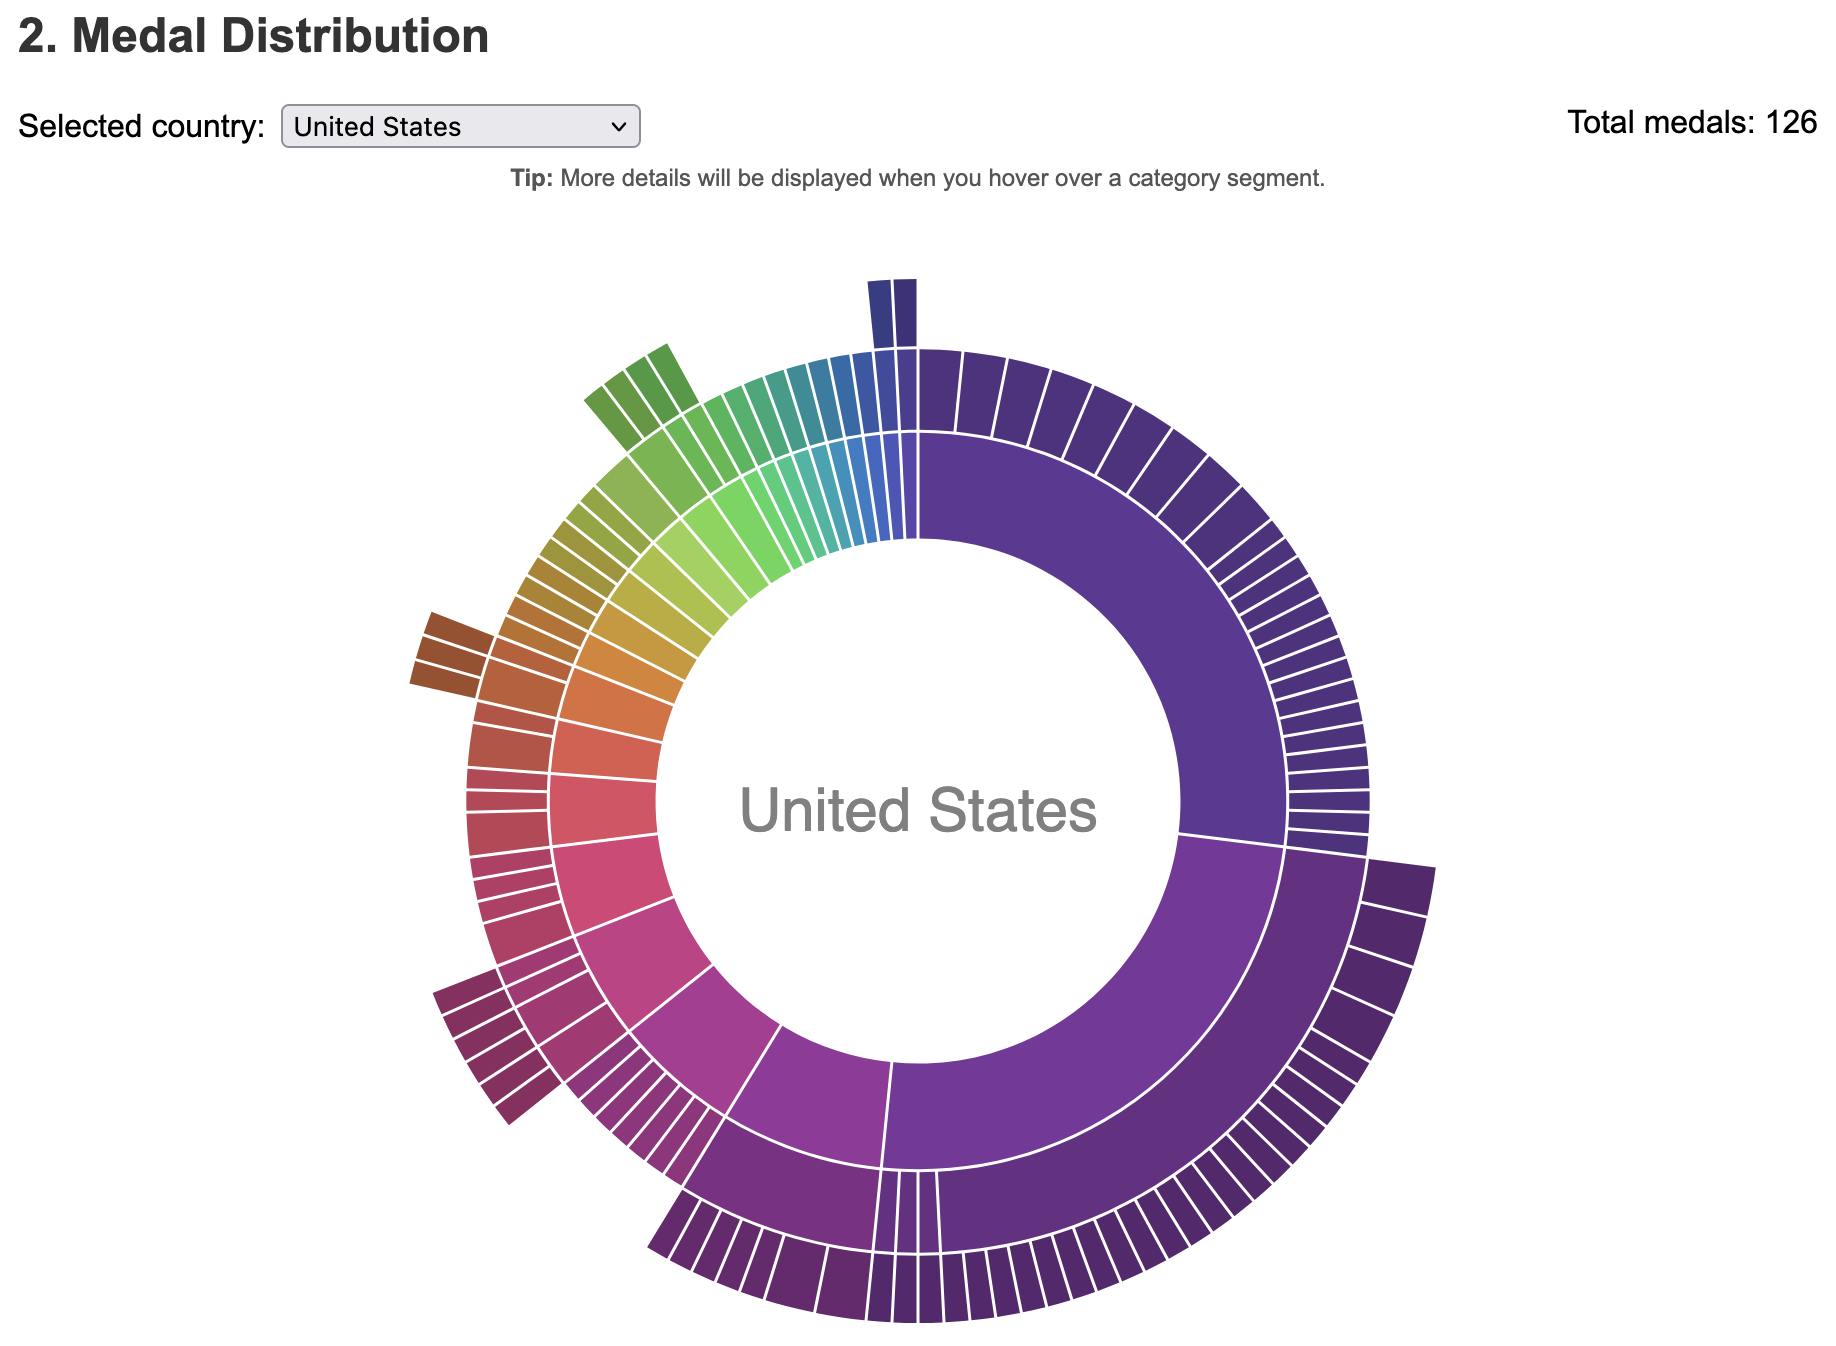
\includegraphics[width=0.5\linewidth]{img/SunBurst_USA.png}
    \caption{Medaillenverteilung der Vereinigten Staaten}
    \label{fig:usa}
\end{figure}

Auf den ersten Blick fällt das Diagramm durch seine vielen Farben auf. Vor allem oben links sind viele verschiedene Farben sichtbar, welche unterschiedliche Sportarten repräsentieren. Das bedeutet, dass die Vereinigten Staaten in vielen unterschiedlichen Sportarten Medaillen gewinnen konnten. Bei genauerer Betrachtung können 26 verschiedenen Sportarten gezählt werden. Weiterhin fällt das Diagramm auf der rechten Seite durch viele violette Farben auf. Große Flächen gleicher Farbe bedeuten, dass ein großer Anteil der Medaillen in der gleichen Sportart gewonnen wurde. Per \textit{Mouse-Hover} über die Kreissegmente werden $26.98\%$ der Medaillen der Kategorie \textit{Athletics} und $24,6\%$ der Kategorie \textit{Aquatics} zugeordnet. Somit stammen $50\%$, also 63 Medaillen, nur allein aus diesen beiden Sportarten. 

% Begründen sie warum Anwendungsfall wichtig für Zielgruppe ist
Die Interpretation dieser Ergebnisse kann je nach Anwender sehr unterschiedlich ausfallen. Da China im Medaillenspiegel Platz zwei hinter den Vereinigten Staaten belegt hat, könnte ein chinesischer Reporter Nachforschungen zu diesem Ergebnis anstellen. Anhand des Medaillenspiegels kann er nur erkennen, dass die Vereinigten Staaten mehr Medaillen gewonnen haben als China und somit sportlich erfolgreicher waren. Mithilfe der Visualisierung kann er aber die Verteilung der Medaillen nach Sportarten und Disziplinen betrachten und argumentieren, dass die Vereinigten Staaten ohne die erfolgreichen Sportler in den Kategorien \textit{Athletics} und \textit{Aquatics} nicht besser als China gewesen wären. Ein Schwimmer könnte das Ergebnis ganz anders interpretieren und würde aufgrund der Dominanz der Vereinigten Staaten in seiner Sportart mit dem Gedanken spielen, sein Training in dieses Land zu verlagern, um von den offensichtlich guten Voraussetzungen zu profitieren. In beiden Fällen hätte ihnen der Medaillenspiegel nicht ausgereicht, um diese Informationen zu erhalten. Erst durch die Visualisierung konnten sie diese Analyse durchführen.

% Diskutieren sie wo Information auch mit anderen hätte gefunden werden
Als Alternative zu dem SunBurst-Diagramm wurden bereits TreeMaps genannt. Diese Visualisierungstechnik kann die Verteilung der Medaillen nach Sportarten und Disziplinen ebenfalls darstellen. Dabei würde die Hierarchie durch ineinander geschachtelte Rechtecke abgebildet werden. Die Farben könnte in gleicher Weise eingesetzt werden. Der wesentliche Unterschied ist die Art der Darstellung der Hierarchie, bei der in der TreeMap ineinander geschachtelten Rechtecke und im SunBurst-Diagramm konzentrische Ringsegmente  als zusammengehörig interpretiert werden müssen. Die meisten Anwender werden Kreis- bzw. SunBurst-Diagrammen schon häufig in ihrem Alltag begegnet sein, sodass diese für sie einfacher zu interpretieren sind als TreeMaps. Der technische Aufwand für die Implementierung dürfte bei beide Visualisierungen ähnlich groß sein.

\subsection{Anwendung Visualisierung Zwei}
% Präsentieren sie einen sinnvollen Anwendungsfall
Der kleine Inselstaat Grenada erzielte bei den Olympischen Sommerspielen 2024 mit zwei Bronzemedaillen das beste Ergebnis in der Geschichte. Aus diesem Grund dürfte die Freude darüber sehr groß gewesen sein. In dem Medaillenspiegel belegt es aber nur Platz 81, da bei diesem Ranking externe Einflussfaktoren, wie zum Beispiel die geringe Einwohnerzahl von gerade einmal $117.000$ Einwohner, nicht in die Bewertung einfließen. Aber aus dieser Perspektive sind zwei Medaillen eine enorme Leistung. Daher sollen die Anwender die gewonnen Medaillen mit demografischen und wirtschaftlichen Einflussfaktoren in Beziehung setzen und die Frage nach der sportlich erfolgreichsten Nation mithilfe dieser alternativen Länderrankings neu beantworten. Die in \autoref{fig:grenada} dargestellte Visualisierung zeigt den Vergleich der Platzierungen von Grenada in den verschiedenen Länderrankings. Dabei wird deutlich, dass Grenada sowohl im Vergleich \enquote{Medaillen pro Einwohnerzahl}, als auch \enquote{Medaillen pro Bruttoinlandsprodukt} zu den erfolgreichsten Ländern gehört. Außerdem können im Hintergrund viele sich kreuzende Linien beobachtet werden. Das bedeutet, dass Länder die im Medaillenspiegel einen guten Platz belegt haben, unter dem Einfluss externer Faktoren nicht mehr so gut bewertet werden. Umgedreht schneiden Länder mit einer schlechten Platzierung im Medaillenspiegel besonders gut in den alternativen Länderrankings ab.

\begin{figure}[!tb]
    \centering
    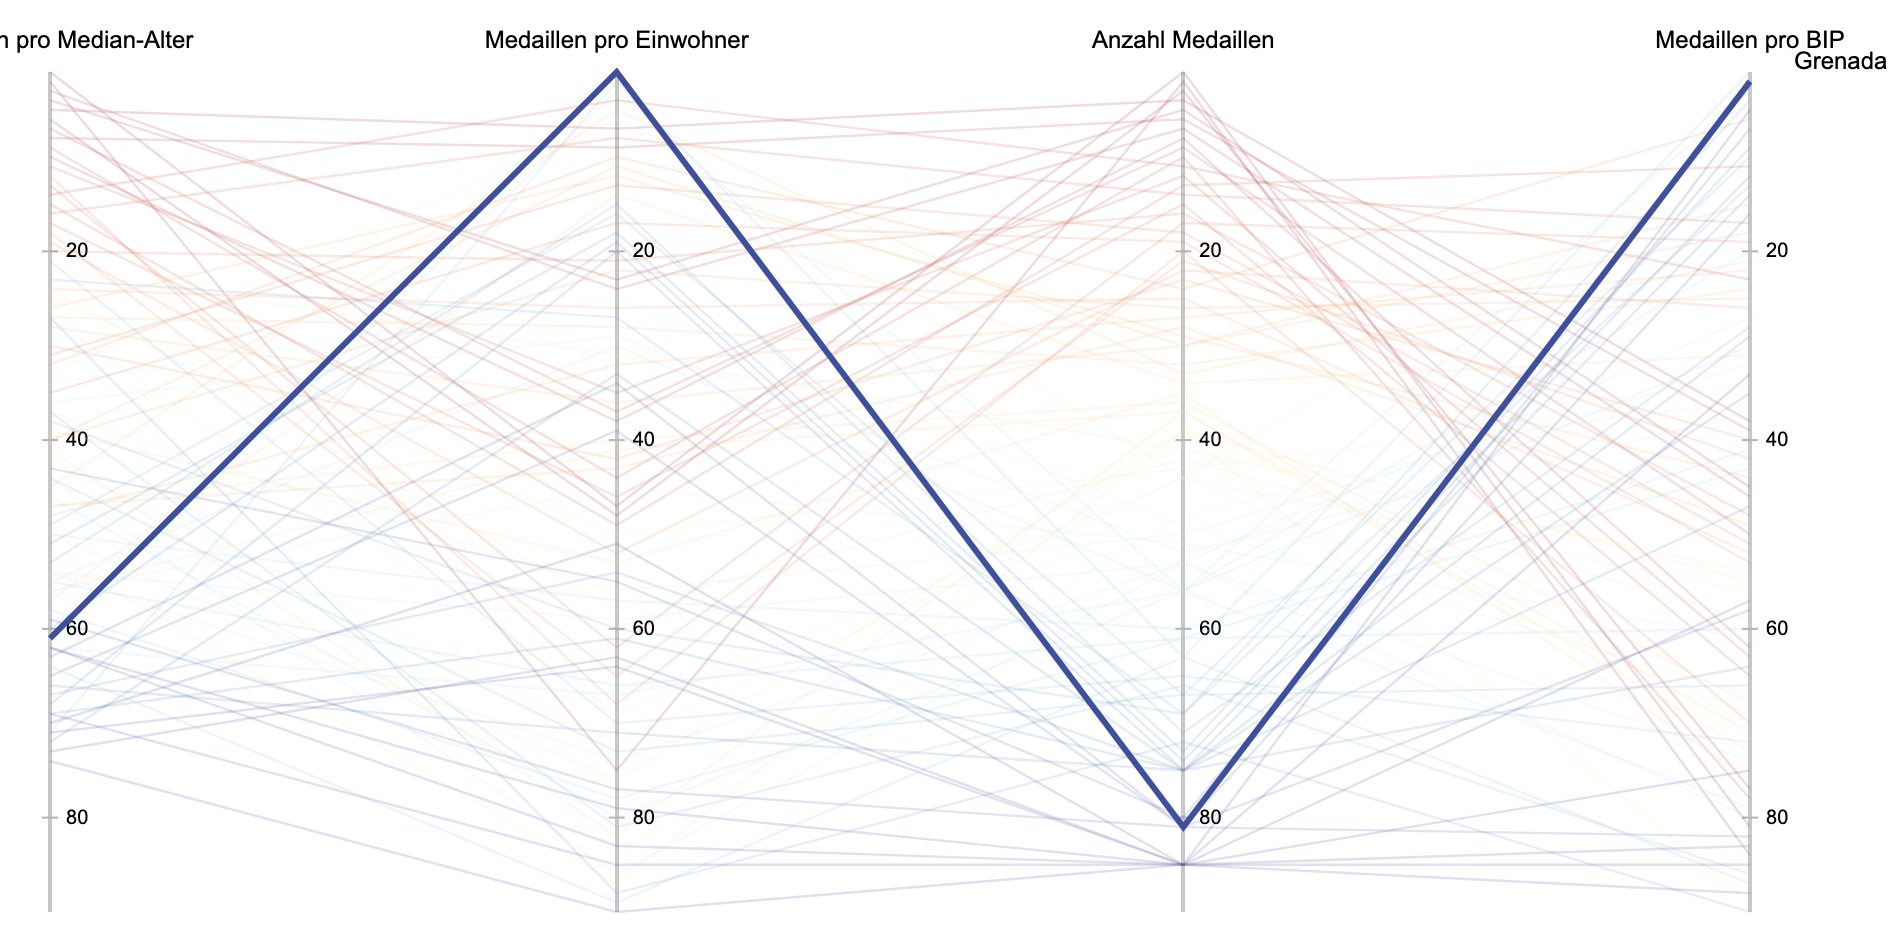
\includegraphics[width=0.5\linewidth]{img/Grenada.png}
    \caption{Grenada in den verschiedenen Länderrankings}
    \label{fig:grenada}
\end{figure}

% Begründen sie warum Anwendungsfall wichtig für Zielgruppe ist
Der bekannte Medaillenspiegel bewertet nur die absolute Anzahl gewonnener Medaillen, wo Grenada mit zwei Medaillen nur einen der hinteren Plätze belegt. Unter diesen Umständen würde niemand Grenada als das sportlich erfolgreichste Land der Olympischen Sommerspiele bezeichnen. Die demografischen und wirtschaftlichen Entwicklungen sind in diesem Land aber ganz anders als zum Beispiel in den Vereinigten Staaten. Aufgrund des viel geringeren Bruttoinlandsprodukt stehen dem Land auch viel weniger finanzielle Mittel für den Sport zur Verfügung. Indem demografische und wirtschaftliche Einflussfaktoren in die Bewertung aufgenommen werden, wird dem sportlichen Erfolg Grenadas mehr Bedeutung gegeben. Dadurch können die Anwender die sportlichen Erfolge einer Nation aus einem anderen Blickwinkel betrachten und die Frage nach der sportlich erfolgreichsten Nation neu beantworten.

% Diskutieren sie wo Information auch mit anderen hätte gefunden werden
In dem beschriebenem Anwendungsfall werden die verschiedenen Länderrankings für ein konkretes Land miteinander verglichen. Dies könnte auch mit einem Scatterplot umgesetzt werden. Jedoch ist die Anordnung der Länderrankings entlang der Achse fest und kann nicht beliebig vertauscht werden. Dadurch ist ein direkter Vergleich von zwei Länderrankings nicht möglich. Die Anordnung der Achsen in den Parallelen Koordinatensystem ist aufgrund des Aufbaus dieser Visualisierung ohne Probleme möglich. Darüber hinaus wurden die sich kreuzenden Linien in der Grafik angesprochen, wodurch allgemeine Änderungen in der Platzierung schnell erkannt werden können. Diese Information kann mit anderen Visualisierungstechniken nicht besser dargestellt werden, als in der kompakten Form in dem Parallelen Koordinatensystem. 

\subsection{Anwendung Visualisierung Drei}
% Präsentieren sie einen sinnvollen Anwendungsfall
Bei der Betrachten des historischen Medaillenspiegels in \autoref{fig:allTime}, sortiert nach dem Kriterium \enquote{All-Time}, können bei dem direkten Vergleich von Polen und Finnland interessante Entwicklungen beobachtet werden. Bei der Darstellung der Medaillenspiegel von Polen fällt eine Reihe gleichfarbiger Zellen ab dem Jahr 1984 auf. Diese sind in orange einfärbt und stellen bei einem Blick auf die Legende zwischen 10 und 19 Medaillen pro Olympiade dar. In der darunterliegenden Zeile sind die Medaillenspiegel von Finnland dargestellt. Dort ist ein dunkler Bereich in den Jahren von 1912 bis 1952. Ab dann werden die Zellen immer heller und im Jahre 2024 ist die Zelle komplett weiß, was bedeutet, dass Finnland bei der letzten Olympiade keine Medaille gewonnen hat.

\begin{figure}[!tb]
    \centering
    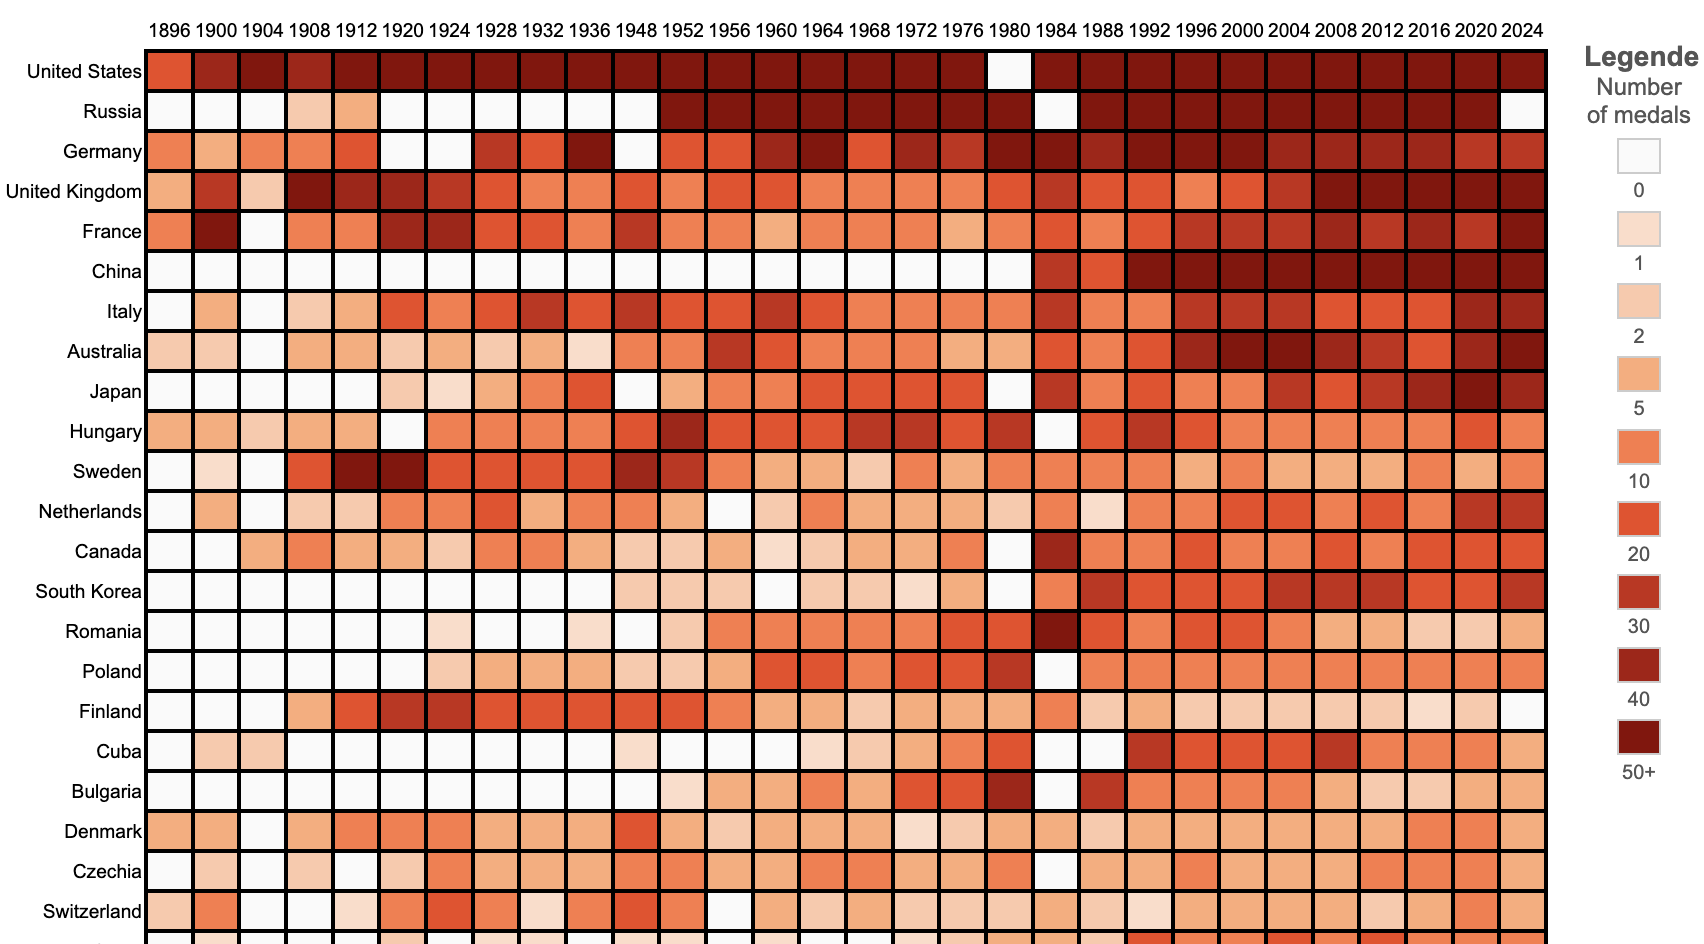
\includegraphics[width=0.65\linewidth]{img/AllTime.png}
    \caption{Historischer Medaillenspiegel}
    \label{fig:allTime}
\end{figure}
% Begründen sie warum Anwendungsfall wichtig für Zielgruppe ist
Die Beobachtung von Polen zeigt, dass dieses Land regelmäßig neue Medaillengewinner beglückwünschen kann und offensichtlich eine gute Talententwicklung hat. Zudem ist davon auszugehen, dass Polen diesen Trend fortsetzen kann und auch bei der nächsten Olympiade Medaillen gewinnen wird. Diese Erkenntnis ist für Sponsoren sehr wichtig, denn diese möchten Sportler und Länder fördern, die gute Aussichten auf Medaillen haben. Anders sieht es für Finnland aus. Dieses Land konnte zum ersten Mal seit 100 Jahren keine Medaille gewinnen. Während andere Länder, wie zum Beispiel Estland, auch keine Medaillen gewonnen haben, war dieses Ereignis bei einem Blick auf die historische Entwicklung von Finnland aber vorhersehbar. Seit 1952 werden die Farben in den Zellen von Finnland immer heller, was eine immer geringere Anzahl an Medaillen bedeutet. Dieses Information ist für Sportler, wie auch Sponsoren sehr wichtig, um sich frühzeitig nach Alternativen umzusehen.

% Diskutieren sie wo Information auch mit anderen hätte gefunden werden
Der historische Medaillenspiegel aller Länder umfasst sehr viele Daten. Um diese auszuwerten und zu analysieren hat sich die HeatMap als optimal erwiesen, da die vielen Informationen sehr kompakt und übersichtlich dargestellt werden können. Die Entwicklungen eines Landes können durch ScatterPlots oder Säulendiagramme visualisiert werden, jedoch können diese Visualisierungen nicht die Entwicklungen aller Länder gleichzeitig darstellen. Die Grafiken wären überladen mit Informationen und sehr unübersichtlich. Ein weiterer Vorteil der HeatMap ergibt sich aus der Kodierung der Werte auf Farbe. Die Farbänderungen sind nach dem Konzept der \textit{Preattentive Recognition} \cite{preAttent} sehr schnell und unterbewusst wahrnehmbar. Deshalb fällt im Beispiel von Polen die lange Reihe gleicher Farbwerte und bei Finnland die immer heller werdenden Zellen sofort auf. Dieser Eigenschaft der Wahrnehmung lässt sich mithilfe der HeatMap am besten ausnutzen.
\section{Verwandte Arbeiten}
% Vorsicht vor "predatory journals" --> Diese zählen nicht als wissenschaftliche Arbeiten (Hier nachschlagen: https://dblp.org/ oder https://dl.acm.org/)
% [x] Führen sie eine kurze Literatursuche in der wissenschaftlichen Literatur zu Informationsvisualisierung und Visual Analytics nach ähnlichen Anwendungen durch.
% [ ] Diskutieren sie mindestens zwei Artikel.
% [ ] Kurze Zusammenfassung verwandter/konkurrierender Arbeiten, die das Problem auf ähnliche Weise lösen 
% [ ] Stellen sie Gemeinsamkeiten und Unterschiede dar.

% Erste Gruppe von Artikeln
% Zweite Gruppe von Artikeln
Nicht nur während der Olympischen Sommerspiele, sondern auch danach interessieren sich Menschen auf der ganzen Welt für die Ereignisse und Ergebnisse. Auch in der Wissenschaft werden die Olympischen Spiele immer wieder thematisiert und analysiert. Ein großer Teil dieser Arbeiten beschäftigt sich mit der Vorhersage neuer Medaillengewinner aufgrund historischer Entwicklungen in einer Sportart. Dabei werden vor allem Methoden der Statistik verwendet. Im Bereich der Informationsvisualisierung gibt es bisher nur wenige  Arbeiten, die eine wissenschaftliche Analyse auf den Daten der Olympischen Sommerspiele durchführen. Auf Kaggle existieren zwar einige Notebooks zu dem Thema, diese untersuchen aber keine wissenschaftliche Fragestellung, sondern stellen willkürliche Diagramme bereit. Trotzdem konnten wir zwei interessante Visual-Analytics-Anwendung finden, die ähnlich zu unserer zentralen Fragestellung, die Bewertungsgrundlage des Medaillenspiegels hinterfragen.

%Zusammenfassung, Gemeinsamkeiten & Unterschiede
\paragraph{Erster Artikel}
In \cite{relWork1} wird festgestellt, dass bestimmte Länder und Kontinente seit jeher einzelne Sportarten dominieren. In der Analyse werden zum Beispiel die Sportarten Tischtennis und Badminton genannt, welche über viele Jahren von China dominiert werden. Außerdem wird der Heimvorteil des Gastgebenden Landes, im Bezug auf den Medaillenspiegel, untersucht. In der Analyse wird eine geringe Steigerung der Anzahl gewonnener Medaillen festgestellt, welche mit der automatischen Qualifikation des Gastgebenden Landes begründet wird.

Diese Visual-Analytics-Anwendung in \cite{relWork1} soll den Anwendern verdeutlichen, dass selbst in einem solchen globalen Sportevent Dominanz und Vorteile existieren. Die Anwender sollen eine neue Perspektive auf die Ergebnisse der Olympischen Spiele erhalten, wobei ihnen die bereitgestellten Visualisierungstechniken unterstützen sollen. Die Daten in \cite{relWork1} werden von einer ähnlichen Quelle geladen, wie die historischen Daten der Olympischen Sommerspiele, welche in dieser Arbeit genutzt werden. Zur Visualisierung der Dominanz eines Landes/Kontinents in einer Sportart wird ein SunBurst-Diagramm verwendet. Diese Entscheidung wird mit der kompakten Darstellungsform begründet, da in dem SunBurst-Diagramm verschiedene Sportarten gleichzeitig dargestellt werden können. Trotzdem werden die verschiedenen Sportarten nicht alle in dem gleichen Diagramm dargestellt, sondern auf fünf Diagramme verteilt. Die Farben repräsentieren hierbei das Land/den Kontinent und die verschiedenen Jahre werden auf die Hierarchie abgebildet. Dieser Unterschied zu dieser Arbeit resultiert aus den verschiedenen Anwendungsaufgaben, welche die Visualisierung unterstützen soll. Zur Darstellung der historischen Medaillenspiegel wird in \cite{relWork1} ein Linien-Diagramm verwendet. In dieser Arbeit wurde dafür eine HeatMap verwendet, da die Zeitreihen verschiedener Länder übersichtlicher dargestellt werden kann. Die Visualisierung in einem Linien-Diagramm mit 200 Linien ist sehr unübersichtlich und konkrete Werte können nicht identifiziert werden. Dieses Problem wird in \cite{relWork1} dadurch gelöst, dass einzelne Länder hervorgehoben werden können. In der HeatMap ist dies von Anfang an möglich. Als dritte Anwendungsaufgabe in \cite{relWork1} wird ähnlich zu dieser Arbeit ein alternatives Länderranking berechnet. Dabei werden die Anzahl gewonnener Medaillen im Verhältnis zu der Anzahl der Athleten gestellt. Als Visualisierungstechnik wird ein ScatterPlot gewählt. Die Bedeutung der Kodierte Position ist bei dieser Visualisierungstechnik nicht intuitiv verständlich. In dieser Arbeit wird daher das mentale Modell des Rankings genutzt und an den Koordinatenachsen eines Parallelen Koordinatensystems abgebildet. Andererseits können in dem ScatterPlot aber sehr einfach \enquote{Ausreißer} identifiziert werden.

%Zusammenfassung, Gemeinsamkeiten & Unterschiede
\paragraph{Zweiter Artikel}
Auch in \cite{relWork2} werden die vergangenen Olympischen Sommerspiele analysiert. Die Anwender sollen dabei Einblicke in die Entwicklungen und Trends erhalten,. Dazu werden einige Fragen formuliert, welche mithilfe unterschiedlicher Visualisierungstechniken beantwortet werden sollen. Als Datenquelle wird der gleiche Datensatz wie in \cite{relWork1} verwendet.

In der ersten Anwendungsaufgabe sollen die Anwender die erfolgreichsten Länder anhand der Anzahl aller jemals gewonnenen Medaillen identifizieren. Dazu wird eine Weltkarte verwendet, in der die verschiedenen Länder mit unterschiedlichen Farben dargestellt werden. Die Farben entsprechen einem Ranking, welches nicht genauer erklärt wird. In dieser Arbeit wird der \enquote{All-Time} Medaillenspiegel nicht dargestellt, sondern nur der Medaillenspiegel der Olympischen Sommerspiele 2024 als Tabelle. Während in der Tabelle die konkrete Platzierung eines Landes leicht abgelesen werden kann, ermöglicht die Darstellung der Weltkarte globale Strukturen zu identifizieren. Beispielsweise sind auf dem Kontinent Afrika viele graue Flächen, welche Länder ohne Olympische Medaillen darstellen. Diese Art der Visualisierung bietet völlig neue Analysemöglichkeiten. In einer anderen Anwendungsaufgabe in \cite{relWork2} werden die historischen Medaillenspiegel der Länder verglichen. Dazu wird ein Linien-Diagramm verwendet, welches aber nur die fünf besten Länder darstellt. Aufgrund dieser Limitierung ist keine adäquate Analyse möglich. In dieser Arbeit wurde für diese Anwendungsaufgabe eine HeatMap verwendet, welche nicht nur die besten fünf Länder, sondern alle Länder darstellen kann. Trendanalysen sind sowohl im Linien-Diagramm durch Analyse des Verlaufs der Linien, als auch in der HeatMap durch unterschiedliche Farben, möglich. Die anderen Anwendungsaufgaben in \cite{relWork2} sind mit denen dieser Arbeit nicht zu vergleichen, weshalb darauf nicht weiter eingegangen wird.

\section{Zusammenfassung und Ausblick}
% [ ] Fassen sie die Beiträge ihre Visualisierungsanwendung zusammen. Wo bietet sie für die Personen der Zielgruppe einen echten Mehrwert.
% [ ] Was wären mögliche sinnvolle Erweiterungen, entweder auf der Ebene der Visualisierungen und/oder auf der Datenebene?

Das Ziel dieser Visual-Analytics-Anwendung war es, die Anwender beim kritischen Hinterfragen, der im Medaillenspiegel dargestellten Ergebnisse, zu unterstützen. Dazu sollten sie sich mit der Fragestellung auseinandersetzen, welches Land das sportlich erfolgreichste bei den Olympischen Sommerspielen 2024 war. Die Visualisierungstechniken helfen ihnen bei der Beantwortung, indem die erzielten Ergebnisse eines Landes aus einer neuen Perspektive darstellen werden. Dazu werden drei verschiedene Visualisierungen genutzt.

Mithilfe der ersten Visualisierung können die Anwender die Verteilung der Medaillen nach Sportarten und Disziplinen analysieren. Dies war mit dem bekannten Medaillenspiegel bisher nicht möglich. Dadurch können nun vielseitig erfolgreiche Länder genauso gut identifiziert werden, wie Länder, die den Großteil ihrer Medaillen nur in einer einzigen Sportart gewonnen haben. Die zweite Visualisierung präsentiert die Erfolge kleinerer Länder in Abhängigkeit von demografischen und wirtschaftlichen Einflussfaktoren. Diese alternativen Länderrankings werden mithilfe eines Parallelen Koordinatensystems vergleichbar gemacht. Den Anwendern könnte das Verhältnis \enquote{Medaillen pro Einwohnerzahl} als Bewertungsmaßstab zwar bekannt sein, aber eine Grafik, welche dieses Ranking im Vergleich zu dem bekannten Medaillenspiegel darstellt, wird in dieser Visual-Analytics-Anwendung neu eingeführt. Die dritte Visualisierung schafft es, den Anwendern Daten über die letzten 120 Jahre kompakt und übersichtlich aufzubereiten. Bereits diese Eigenschaft ist ein großer Mehrwert für Analysen rund um die Olympischen Sommerspiele. Zur Beantwortung der Fragestellung werden den Anwendern mithilfe von Farben Trends und Entwicklungen hervorgehoben, welche ohne die Visualisierung nicht erkennbar wären.

Aufgrund der verschiedenen Interaktionsmöglichkeiten können die Anwender die Visualisierungen nach ihren persönlichen Vorlieben verändern, um die, für sie am besten geeignete Ansicht zum Beantworten der Fragestellung, zu erhalten.

Die verwendeten Datensätze enthalten neben den Informationen über die Medaillen auch konkrete Daten von den erzielten Leistungen der Sportler. Dadurch könnte zum Beispiel die Abstände zwischen den Erstplatzierten untersucht werden. Die Anwendungsaufgaben könnten dann um die Frage nach dem sportlich erfolgreichsten Sportler erweitert werden. Andererseits ermöglicht die Visualisierung der Weltkarte in \cite{relWork2} völlig neue Analysemöglichkeiten. Dadurch könnte die Frage nach globalen Tendenzen beantwortet werden. 

\section*{Anhang: Git-Historie}
\begin{verbatim}
* 1ed2fec	2025-09-19	add chap 7 and minor changes to chap 5,6
* 818d1ba	2025-09-19	Add chap 4
* fbf2be9	2025-09-18	add chap 5
* b2106cc	2025-09-17	complete chap 2 and refactor chap 1-3
* 3a13928	2025-09-16	add discussion for vis-3 and interactions
* bab2051	2025-09-15	add discussion for vis-2
* d2bd7d1	2025-09-15	add discussion for vis-1
* 281af62	2025-09-14	update chap 1,2
* 9bde4f6	2025-08-01	add chap 1-3
| *   d102744	2025-09-12	Merge branch '15-verbesserte-interaktionen-und-ui' into 'main'
| |\  
| | * be9ced3	2025-09-12	Fehler und Warnungen entfernt
| | * 5d1fc27	2025-09-12	sort heatmap by medaltabl or overall ranking
| | * 29c6d77	2025-09-11	Länder-Normalisierung angepasst
| | * 2a7b42d	2025-09-11	sticky Legende, highlight row/col
| | * 696e225	2025-09-11	Remove checkboxes and enable Click to hightlight
| | * cb1d1a7	2025-09-11	show medals in medal-dist
| | * 85b2a3f	2025-09-10	more infos at medal distribution
| | * 67b86fe	2025-09-10	collapse medaltable and change medalTable Col-Names
| | * 5a6383e	2025-09-10	add link to top
| |/  
| *   2da8ad7	2025-09-10	Merge branch '11-sunburst-schoen-machen' into 'main'
| |\  
| | * 5d79eb6	2025-09-10	improve colors for sunburst
| | *   e005042	2025-09-10	Merge branch 'main' into 11-sunburst-schoen-machen
| | |\  
| | |/  
| |/|   
| * |   5754273	2025-09-10	Merge branch '14-fix-dateiendung-datenquelle' into 'main'
| |\ \  
| | * | b157e35	2025-09-10	change file-format
| |/ /  
| * |   019d669	2025-09-10	Merge branch '13-datenquelle-aendern-und-modell-anpassen'
                            into 'main'
| |\ \  
| | * | 47ceb56	2025-09-10	update pre2024 dataset and model
| | * | 45484d5	2025-09-10	update 2024 dataset and model
| |/ /  
| * |   bc22726	2025-09-10	Merge branch '12-noc-anstelle-von-team-verwenden' into 'main'
| |\ \  
| | * | b4151f9	2025-09-10	nocToCountry Mapping + Visualisierungen an NOC angepasst
| | * | 0d3dc21	2025-09-09	.team durch .noc ersetzt
| |/ /  
| | * 98e2032	2025-09-10	improve catgeories and design
| |/  
| *   259f669	2025-09-09	Merge branch '10-heatmap-fuer-entwicklung-medaillengewinner
                        -ueber-die-zeit' into 'main'
| |\  
| | * 5e5319f	2025-09-09	Fix: HeatMao-Farbskale mit diskreten Werten für besser
                        Unterscheidung zw. 0 und 1 Medaillen
| | * 6f4ad0f	2025-09-09	Order teams by medal_table
| | * 74de043	2025-09-08	Fix: automatische Breite + Legende (oben) + Darstellung
                        alle Länder und Jahre
| | * 7665ef3	2025-09-08	Fix: Überschneidung der Tip und die Legende bei HeatMap
                        + dynamische höhe
| | * 9c576c7	2025-09-08	Schneller Datenaufbereitung + Team-Normalisierung
                        (Cuba-1 bzw. Cuba-2 zu Cuba)
| | * 33ed523	2025-09-08	Legende für HeatMap
| | * b4db102	2025-09-08	HeatMap hinzugefügt (Limited Data)
| |/  
| *   e8fdf1a	2025-09-06	Merge branch '9-interaktion-tabelle-parallele-koordinaten'
                        into 'main'
| |\  
| | * 4e83c4e	2025-09-06	Interaktion: Medallienspiegel und parallele Koordinaten
| |/  
| *   032b9a7	2025-09-05	Merge branch '8-interaktion-tabelle-verteilung'
                        into 'main'
| |\  
| | * 02cf735	2025-09-05	Interaktion: Sprung von Medaillenspiegel zur
                        Medaillenverteilung des entsprechenden Landes
| |/  
| *   461cd4f	2025-09-04	Merge branch '6-paralleles-koordinatensystem-fur-qualitative
                        -faktoren-implementieren' into 'main'
| |\  
| | * 628d8ea	2025-09-04	Anpassung der Zahlendarstellung der PC-Hilfstabelle
| | * 844f022	2025-09-04	Umschaltung zw. tatsächlich relative
                        (Medaillen / Pop, GDP, Age)
| | * c0b08c4	2025-09-03	rank after medal/value and remove countries (EOR,AIN)
| | * d3b5b41	2025-09-03	repositioned info-text
| | * 1272edf	2025-09-01	Hinweis bearbeitet
| | * c98505d	2025-09-01	parallele Koordinaten-Plot implementiert
| |/  
| *   00c4790	2025-08-27	Merge branch 'update-elm-imports' into 'main'
| |\  
| | * 63674d6	2025-08-27	update elm.json
| |/  
| *   aed2055	2025-08-27	Merge branch '4-medaillenverteilung-nach-sportart
                        -implementieren' into 'main'
| |\  
| | * b7de78c	2025-08-27	Hover und CheckBox Update hinzugefügt
| | * 7884555	2025-08-27	SBModell hinzugefügt
| | * e7c0077	2025-08-27	Sunburst-Visualisierung hinzugefügt
| |/  
| *   95524b2	2025-08-20	Merge branch '3-datesatz-anknupfen' into 'main'
| |\  
| | * df90f5d	2025-08-20	Daten gefiltert und die Sortierung angepasst
| | * 53e5af3	2025-08-20	Variablen umbennen
| | * aeafaa1	2025-08-18	Sortierung nach Gold -> Gesamt -> Silber -> Bronze
| | * cd03f80	2025-08-18	Umbenennung auf konsistente englische Bezeichner
| | * 5f46517	2025-08-18	Daten für das Jahr 2024 gefiltert
| | * 01afb13	2025-08-18	Datensatz eingebunden und in Medaillenspiegel geladen
| | * bea3047	2025-08-18	Weiter-Button hinzugefügt
| |/  
| *   b66ee1d	2025-08-17	Merge branch '2-medaillenspiegel-implementieren' into 'main'
| |\  
| | * b03b743	2025-08-17	Medaillenspiegel mit Mockdaten implementiert
| |/  
| * 1886b56	2025-08-09	Update .gitlab-ci.yml file
| * 61a0f43	2025-08-09	Merge branch '1-startseite-implementieren' into 'main'
|/| 
| * 06f4df1	2025-08-09	Grundstruktur der Startseite mit den Hauptkomponenten
                        implementiert
|/  
* 74f7514	2025-08-01	add source-files for report
* f24a31c	2025-07-02	edit pipline (fix)
* ab2c866	2025-07-02	Hello World example project
* 96a31b1	2025-07-01	Add .gitlab-ci.yml
* 750e22c	2025-07-01	Initial commit
\end{verbatim}

\printbibliography

\end{document}

%%%
% Zwischenstände ab Ende Juli bis Mitte August senden
% -> Hinneburg ist im Urlaub (5.-12.09.)